%!TEX root = ../Main.tex

\chapter[expVIP]{expVIP: a customisable RNA-seq data analysis and visualisation platform.}
\label{cha:exp}


\section{Background.}



%Describe the list of previously published expression experiments and how they can potentially be used as a framework for new experiments.  

%Co-expression of homoeologus varies from triplet to triplet \citep{Pfeifer2014}
%The silencing is mostly regulated by epigenetic changes as the hybridization events are recent.  \citep{Bottley2006}


%\begin{table}

%\caption{Studies included in expVIP for wheat}
%\label{tab:exp:studysDetails}

%\end{table}

\subsection{Alternative expression browsers.}
\label{exp:alternative}
%Expression experiments are done routinely in model organisms, such as arabidopsis.

To the best of my knowledge, the only alternative expression browser developed for specifically for wheat is WheatExp \citep{Pearce2015b}. 
This expression browser contains information of 6 studies from diploid, tetraploid and hexaploid wheat. 
The studies were selected to be complementary among them; " a broad study of five different tissues across multiple timepoints \citep{Choulet2014}, a study of seedling photomorphogenesis \citep{Fox2014}, a study of drought and heat stress in wheat seedlings \citep{Liu2015}, a study of wheat grain layers at a single timepoint \citep{Pearce2015}, a senescing leaf timecourse \citep{Pearce2014} and a timecourse of different grain tissue layers during development \citep{Pfeifer2014}".
The expression quantification is produced by aligning to the gene transcripts using BWA \citep{Li2010}, and the counts are extracted with HTSeq \citep{Anders2015}. 
The Expression Atlas from \acrshort{ebi} is a public resource that collects expression experiments of several species \citep{Petryszak2016}. 
The samples are processed automatically from the reads deposited ArrayExpress \citep{Kolesnikov2015}, containing data from microarrays and RNA-Seq.
The studies included are manually curated and annotated with the relevant ontologies. 
As of September 2016, 202 differential and 82 base experiments had been included. 
The visualisation is designed to explore each gene individually, showing all the related ontologies and details on the expression by factor, or by pairs of factor on a heatmap. 
The quantification is calculated with HTSeq \citep{Anders2015}, from alignments produced with Tophat \citep{Ling2013}.

\unsure{introduce BioGPS. It is not wheat related, but is feature rich. }


\subsection{Public wheat RNA-Seq experiments.}

Table of experiments to include 
%!TEX root = ../../Main.tex
\begin{sidewaystable}
\caption{Studies with RNA-Seq replicates, sequenced with Illumina, at the time when expVIP was under development.} 
\label{tab:exp:studiesDetails}
\footnotesize
\begin{tabular}{p{2cm}p{3cm}p{7.4cm}p{10.1cm}}
\toprule
 Study Id & Summary of study  & Brief SRA description  & Manuscript  \\
\midrule
 DRP000768 & Phosphate starvation in roots and shoots & Transcriptome profiles of wheat variety Chinese Spring (CS) in response to Pi starvation (-P) for 10 days. & Characterisation of the wheat (\textit{Triticum aestivum L.}) transcriptome by \textit{de novo} assembly for the discovery of phosphate starvation-responsive genes: gene expression in Pi-stressed wheat \citep{Oono2013}. \\
 ERP003465 & fusarium head blight infected spikelets & Near isogenic wheat lines, differing in the presence of the \textit{Fusarium graminearum} FHB-resistance QTL Fhb1 and Qfhs.ifa-5A, under disease pressure (30 and 50 hai) as well as with mock-inoculation  & Quantitative trait loci-dependent analysis of a gene co-expression network associated with Fusarium head blight resistance in bread wheat \textit{Triticum aestivum L.}. \citep{Kugler2013}.  \\
 ERP004505 & grain tissue-specific developmental timecourse & Analysis of the cell type specific expression of homeologous genes in the developing wheat grain & Genome interplay in the grain transcriptome of hexaploid bread wheat \citep{Pfeifer2014}. \\
 SRP004884 & flag leaf downregulation of GPC & Wild type bread wheat plants and GPC RNAi plants 12 days after anthesis  & Effect of the down-regulation of the high Grain Protein Content (GPC) genes on the wheat transcriptome during monocarpic senescence \citep{Cantu2011b}. \\
 SRP013449 & grain tissue-specific developmental timecourse & Transcriptomes of the aleurone and starchy endosperm tissues of the wheat seed (\textit{Triticum aestivum}) at time points critical to the development of the aleurone layer of 6, 9 and 14 days post anthesis. & Gene expression in the developing aleurone and starchy endosperm of wheat \citep{Gillies2012}. \\
 SRP017303 & stripe rust infected seedlings & Pool of stripe rust infected wheat leaves & Genome analyses of the wheat yellow (stripe) rust pathogen \textit{Puccinia striiformis f. sp. tritici} reveal polymorphic and haustorial expressed secreted proteins as candidate effectors \citep{Cantu2013}. \\
 SRP022869 & \textit{Septoria tritici} infected seedlings   & Molecular mechanisms underlying the interplay between fungal pathogenicity and host responses at specific growth phases and the factors triggering disease transition. & Transcriptional Reprogramming of Wheat and the Hemibiotrophic Pathogen \textit{Septoria tritici} during Two Phases of the Compatible Interaction \citep{Yang2013}. \\
 
 \bottomrule
\end{tabular}
\end{sidewaystable}

\begin{sidewaystable}
\footnotesize
\begin{tabular}{p{2cm}p{3cm}p{7.4cm}p{10.1cm}}
\toprule
 Study Id & Summary of study  & Brief SRA description  & Manuscript  \\
\midrule
SRP028357 & shoots and leaves of nulli tetra group 1 and group 5 & RNAseq of nulli-tetrasomic wheat lines (shoots and leaves & Patterns of homoeologous gene expression shown by RNA sequencing in hexaploid bread wheat \citep{Leach2014}. \\
 SRP029372 & grain tissue-specific developmental timecourse & Gene expression profiling of morphological stage of developing wheat grain & Evaluation of Assembly Strategies Using RNA-Seq Data Associated with Grain Development of Wheat (\textit{Triticum aestivum L.}; \citealt{Li2013}). \\
 SRP038912               & comparison of stamen, pistil and pistilloidy expression & Transcriptional profiling of pistillody stamen, pistil and stamen in wheat line HTS-1 & Pistillody mutant reveals key insights into stamen and pistil development in wheat (\textit{Triticum aestivum L.}; \citealt{Yang2015}). \\
 SRP041017 & stripe rust and powdery mildew timecourse of infection in seedlings & Transcriptome Divergence and Overlap for Wheat in Response to Stripe rust and Powdery Mildew Pathogen Stress & Large-scale transcriptome comparison reveals distinct gene activations in wheat responding to stripe rust and powdery mildew. \citep{Zhang2014}. \\
 SRP041022  & developmental time-course of synthetic hexaploid & RNAseq of three tissues of nascent allohexaploid wheat and its following generations, their progenitors, and Chinese Spring & mRNA and Small RNA Transcriptomes Reveal Insights into Dynamic Homoeolog Regulation of Allopolyploid Heterosis in Nascent Hexaploid Wheat \citep{Li2014}). \\
 ERP008767 & grain tissue-specific expression at 12 days post anthesis & Inner pericarp, outer pericarp and endosperm layers from developing grain of bread wheat cv. Holdfast at 12 days post-anthesis. & Heterologous expression and transcript analysis of gibberellin biosynthetic genes of grasses reveals novel functionality in the \textit{GA3ox} family \citep{Pearce2015}. \\
 SRP045409 & drought and heat stress time-course in seedlings & RNAseq of 1-week old wheat seedling leaves subjected to drought stress, heat stress and their combination before (0h) and after stress (1h or 6h) & Temporal transcriptome profiling reveals expression partitioning of homeologous genes contributing to heat and drought acclimation in wheat (\textit{Triticum aestivum L.}; \citealt{Liu2015}). \\
  INRA-RNAseq (ERP004714) & developmental time-course of Chinese Spring & Whole transcriptome sequencing of wheat 3B chromosome  & Structural and functional partitioning of bread wheat chromosome 3B \citep{Choulet2014}. \\
 SRP056412 & grain developmental timecourse with 4A dormancy QTL & This study was to identify candidate genes underlying the 4AL QTL for grain dormancy in wheat. RNA was sequenced from pooled NILs segregating for the QTL & Transcriptomic analysis of wheat near-isogenic linesidentifies  \textit{PM19-A1} an \textit{A2} as candidates for a major dormancy QTL \citep{Barrero2015} \\
\bottomrule
\end{tabular}
\end{sidewaystable}


\subsection{Expression quantification with Kallisto.}
\label{exp:kallisto}
Differential expression experiments try to elucidate which genes change under different conditions. 
To do that, a quantification of the levels of expressions is needed. 
When using RNA-Seq, the expression analysis usually consists on: aligning the reads to the genome or transcriptome reference and quantify the expression according to how many reads map to a region. 
However, this process usually takes around 6 hours per sample. 
Aligners such as \texttt{bwa} or \texttt{bowtie} produce a detailed alignment of each read, which is useful find polymorphisms (see Chapter \ref{yr15}) or to find novel alternative splices \citep{Trapnell2012}. 

For expression analysis only the count of how many reads with a transcript is required, calculating the best local alignment and the output of each read is unnecessary. 
\verb|Kallisto| is a tool that generates an index based on overlapping k-mers (sequences of size $k$), which are connected sequentially to represent each transcript  on a \gls{tdbg}. 
For alternative splicings of the same gene, were some sequence overlap between transcripts, the connections produce two different sets of connections between k-mers. 
The k-mers on each read are then used to find the compatible transcripts across the T-DBG and those are counted. 
Finally, the program estimates the abundance of the transcript in the sample (Figure \ref{fig:exp:kallisto}; \citealt{Bray2016}).  


\begin{figure}
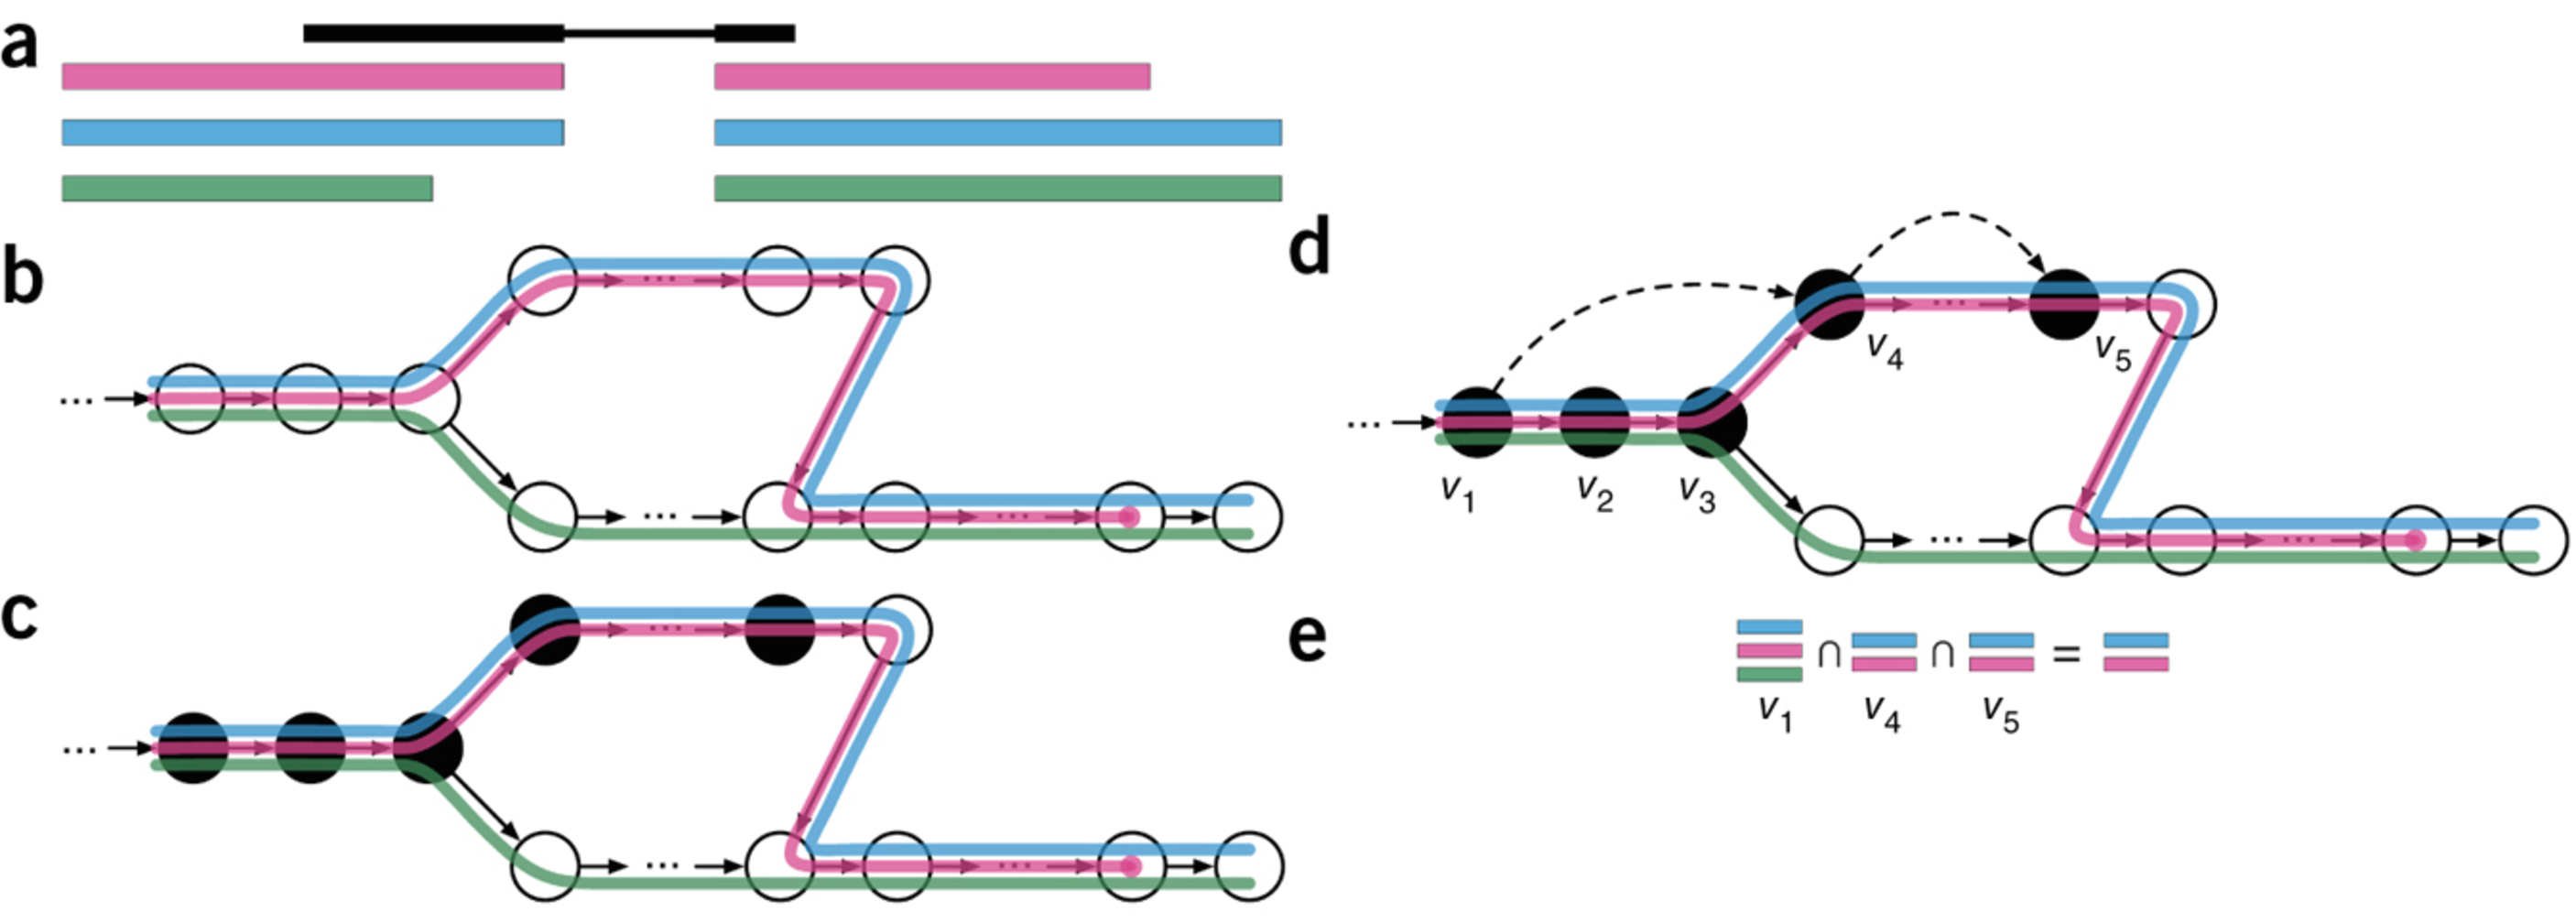
\includegraphics[width=1\textwidth]{LitReview/Figures/kallisto.pdf}
\caption[Overview of kallisto.]{"Overview of kallisto. The input consists of a reference transcriptome and reads from an RNA-seq experiment. (a) An example of a read (in black) and three overlapping transcripts with exonic regions as shown. (b) An index is constructed by creating the transcriptome de Bruijn Graph (T-DBG) where
nodes (v1, v2, v3, ... ) are k-mers, each transcript corresponds to a colored path as shown and the path cover of the transcriptome induces a k-compatibility class for each k-mer. (c) Conceptually, the k-mers of a read are hashed (black nodes) to find the k-compatibility class of a read. (d) Skipping (black dashed lines) uses the information stored in the T-DBG to skip k-mers that are redundant because they have the same k-compatibility class. (e) The k-compatibility class of the read is determined by taking the intersection of the k-compatibility classes of its constituent k-mers" \citep{Bray2016}.}
\label{fig:exp:kallisto}
\end{figure}


\subsection{Relational databases.}
A Relational database is a set of structured tables that have relationships between each other. 
The tables correspond to the data that is essential for the represented concept (domain).
For example, in a table representing several species, the common name and the scientific name belong to the same domain (ie name: Bread wheat; scientific name \textit{Triticum aestivum}). 
Tables in the same relational database form relationships between each other. 
Continuing with the example, a species can have several scientific studies related to them. 
The domain of a study can be formed by the accession, a title, a corresponding manuscript and the species it is concerned with. The two tables can be connected by the usage of a common ID signifying the species. It is therefore common practice to create an extra column containing unique integer values, to act as connecting keys between two or more tables. Such a column is defined as the primary key of the table; although, strictly speaking, any set of columns whose combination of values is unique for each row can act as primary key. 
In our example an extra \texttt{id} column is added allowing to create a stable relationship between the \verb|Species| and the \verb|Studies| tables.
 (Figure \ref{fig:expvip:miniER}; \citealt{Codd1970}).
The tables \ref{exp:tab:species} and \ref{exp:tab:studies} have the content of their corresponding domains. 

\begin{figure}
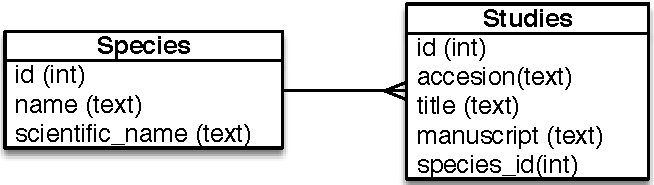
\includegraphics{expVIP/Figures/miniER.pdf}
\caption[Example of a relationship between tables.]{Example of a relationship between tables. The tables Species and Studies are related. Each study has one species and each species can have several studies.}
\label{fig:expvip:miniER}
\end{figure}

\begin{table}
\caption[Species]{Example content for the table \texttt{species}}
\label{exp:tab:species}
\centering
\begin{tabular}{rll}
\toprule
   id & name                          & scientific\_name                                         \\
\midrule
    1 & Bread wheat                 & Triticum aestivum                                     \\
    2 & Yellow rust                 & Puccinia striiformis              \\
    3 & wheat and rust & T.aestivum,S.tritici  \\
\bottomrule
\end{tabular}

\end{table}

\begin{table}
\caption[Studies]{Example content for the table \texttt{studies}}
\label{exp:tab:studies}
\centering
\begin{tabular}{rllr}
\toprule
   id & accession                                          & manuscript                              &   species\_id \\
\midrule
    1 & DRP000768                                          &  10.1186/1471-2164-14-77          &            1 \\
    2 & ERP003465                                          & 10.1186/1471-2164-14-728            &            1 \\
    3 & ERP004505                                          &  10.1126/science.1250091          &            1 \\
    4 & SRP004884                                          & 10.1186/1471-2164-12-492            &            1 \\
    5 & SRP013449                                          &  10.1111/j.1467-7652.2012.00705.x &            1 \\
    6 & SRP017303                                          & 10.1186/1471-2164-14-270            &            2 \\
    7 & SRP022869                                          &  10.1371/journal.pone.0081606     &            3 \\
\bottomrule
\end{tabular}

\end{table}

\subsection{SQL.}
\gls{sql} is a common language to retrieve information from relational databases. 
\acrshort{sql} has operations to select columns and rows, join tables, group repeated values and order the results. 
Those simple operations are enough to retrieve information between tables \citep{Oracle2014}. 
The following list shows a brief description of some commands  that can be used to build a query.  

\begin{description}
\item[\texttt{SELECT <EXPRESSIONS> }]. A list of columns or an expression that will be displayed, separated by commas (\texttt{,}). To display all the columns, the \texttt{*} character  all the columns in the table. The order of the columns will be the same as the order given in this part of the command
\item[\texttt{FROM <TABLE>}]. follows the column names to add a list of tables to select from.
\item[\texttt{JOIN <TABLE> ON <EXPRESSION> }]. is used to join the table from the left side of the statement with the \texttt{<EXPRESSION>} given after the \texttt{ON} clause.  
\item[\texttt{WHERE <EXPRESSION>}] filters the rows by the \texttt{<EXPRESSION>}
\item[\texttt{ORDER BY <COLUMNS>}]. The rows will be sorted by the natural order of the given \texttt{<COLUMNS>}.  
\item[\texttt{GROUP BY <COLUMNS>}]. The rows are merged by the columns stated. This can be used to get an unique set of values and apply a function to all the rows that have the same value, as a count.
\end{description} 

Expressions can be values, operators or functions like:

\begin{description}
\item[\texttt{COLUMN}] The value of a column. 
\item[ \texttt{<EXPRESSION> = <EXPRESSION>}] \texttt{TRUE} when the left and right \texttt{<EXPRESSION>} are equal. \texttt{FALSE} otherwise 
\item[ \texttt{<EXPRESSION> > <EXPRESSION>}] \texttt{TRUE} when the left  \texttt{<EXPRESSION>} is greater than the  right \texttt{<EXPRESSION>} are equal. \texttt{FALSE} otherwise 
\item[ \texttt{<EXPRESSION> < <EXPRESSION>}] \texttt{TRUE} when the left  \texttt{<EXPRESSION>} is less than the  right \texttt{<EXPRESSION>} are equal. \texttt{FALSE} otherwise
\item[ \texttt{COUNT(*)}] The count of rows that have the same values, as selected in the \texttt{GROUP BY} clause.
\end{description}

A simple query to join the  \texttt{species} and \texttt{studies} tables and displaying only the species name, scientific name and accession of the study is shown in Listing \ref{exp:lst:joinExample}. 
The results of the query are in Table \ref{exp:tab:joinExample}. 

\begin{code}[language=sql, label=exp:lst:joinExample,caption=Join example query]
SELECT 
	species.name, 
	species.scientific_name, 
	studies.accession, 
FROM species
JOIN studies on species.id = studies.species_id;
\end{code}

\begin{table}[h!]

\caption[Join example]{Join of the \texttt{species} and \texttt{studies} table. }
\label{exp:tab:joinExample}
\centering
\begin{tabular}{lll}
\toprule
 name                          & scientific\_name                                         & accession                                                                       \\
\midrule
 Bread wheat                 & Triticum aestivum                                     & DRP000768                                          \\ 
 Bread wheat                 & Triticum aestivum                                     & ERP003465                                          \\ 
 Bread wheat                 & Triticum aestivum                                     & ERP004505                                          \\ 
 Bread wheat                 & Triticum aestivum                                     & SRP004884                                          \\ 
 Bread wheat                 & Triticum aestivum                                     & SRP013449                                          \\ 
 Yellow rust                 & Puccinia striiformis            & SRP017303                                          \\ 
 wheat and rust & T.aestivum,S.tritici & SRP022869                                          \\ 
\bottomrule
\end{tabular}

\end{table}


The relationships between tables can be of the following types:

\begin{description}
\item[one-to-one.] When rows on a table can be related to a row in a second table. On the diagrams they are represented by a straight line.
\item[many-to-many.] Rows on a table can have many corresponding rows in a second table, resented with lines with whiskers on both sides of the line.  
\item[one-to-many.] Rows on a table can be related to many rows on the second table, represented with whiskers only on one side of the line. 
\end{description}

An important feature of a database is the ability to store the data consistently.
A transaction is a set of related operations that need to be performed at the same time; as such, it needs to follow the principles of \gls{acid} \citep{Haerder1983}.


\begin{description}
\item[Atomicity.] All the operations or none have to be performed. If any of them fails or an error happens while the transaction is executed, the data has to be restored to the original status. 
\item[Consistency.] The changes in the database have to be valid before and after the transaction. 
\item[Isolation.] If more than one transaction is being executed at the same time, the result must be the same as if the transactions were executed one after the other. 
\item[Durability.] The result of the transaction is stored even if the server is restarted.
\end{description}  

\unsure{Add explanaiton of inserts. }

Several \gls{rdbms} implement \acrshort{sql}, with various levels of compliance to the standard and different licenses.  
A popular \acrshort{rdbms} is \texttt{MySQL}.
From the beginning \texttt{MySQL} aimed to be a lightweight and easy to install open source product \citep{Oracle2014}. 
This characteristics made it popular on the web and it is currently the \gls{rdbms} behind ensembl! \citep{Flicek2012}. 

\subsection{Model-View-Controller}

\begin{SCfigure} 
  \centering
  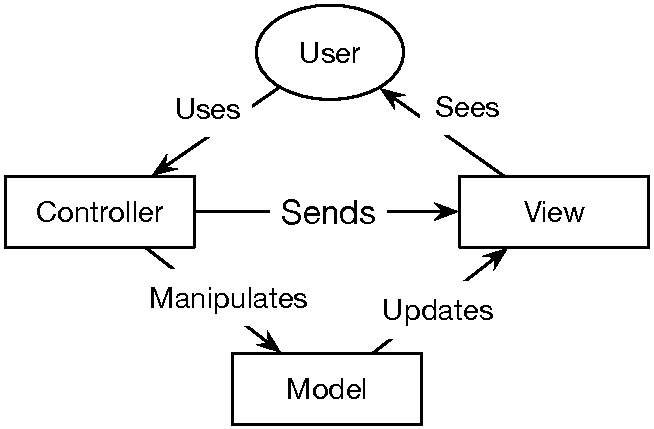
\includegraphics[width=0.7\textwidth]{LitReview/Figures/MVC.pdf}
  \caption{\acrshort{mvc} interaction between components.}
  \label{fig:poly:mvc}
\end{SCfigure}
The \gls{mvc} is a metaphor to isolate the user interactions from the underlying data. 
The models hold the data on logical their domains.
The views contain the layout on how the models are displayed to the user.
The controllers receive the requests from the users and modify the models hold the data as mapped to their logical domains accordingly and send a view back for display. 
The \acrshort{mvc} metaphor allows the development of independent parts of the system and helps to structure the underlying representation of the domains.  (Figure \ref{fig:poly:mvc}; \citealt{Krasner1988}).

\gls{ror} is a framework to develop web applications heavily influenced by the \acrshort{mvc} metaphor. 
It is based on the Rails language and provides several tools designed to facilitate development, such as automated tasks designed to create models with their corresponding views and controllers. 
On the top of that, it provides the tools to manage the connection and queries to the \acrshort{rdbms}, allowing the developer to focus on functionality \citep{RailsGuide2016}. 

\subsection{Data visualisation}

In the last couple of decades the amount of information available in any given field has been growing exponentially, in part thanks to the internet. 
A standing challenge is therefore to produce tools that help interpretation. 
An effective way to communicate large amount of data is through visualisation, but it has to have the following properties to be usable \citep{Myatt2011}:

\begin{description}
\item[Time to learn.] The user needs to take little time to learn how to use the system to extract the information they need. Also, all the features should be easy to find.
\item[Performance.] The tool needs to be quick to access and transform the visualisation as the user requests.
\item[Accuracy.] The tool has to perform as the user expects, so if the tool is prone to make users commit mistakes, it is not accurate. 
\item[Memorability.] Once the user learns to use the system, is it easy to remember how to use it? Systems that change their interface often, or between windows are not as easy to remember. 
\item[Satisfaction.] The user responds positively to the use of the system and the time is spent actually exploring the data, rather than trying to make the system work. 
\end{description}

\subsection{Aims}
\label{exp:aims}
The aims of expVIP are to:
\begin{enumerate}
\item Integrate RNA-Seq experiments from several sources in a single database (Section \ref{exp:DB}). 
\item Automate the calculation of the expression values and load them in to the database (Section \ref{exp:pipeline}).
\item Produce a usable visualisation for said expression values (Section \ref{exp:gui}).
\item Make the system available to the community (Section \ref{exp:gui}).
\end{enumerate}

The software developed in this chapter is published in \cite*{Borrill2016}. 

\section{General design}

One of the main objectives of expVIP is to make the public expression datasets easily accessible and explorable for the target community (currently wheat, but not limited to it). 
A web interface is an effective way to reach a global audience. 
A web service requires to have a server to run the application, and a browser to connect to the server and display the application to the user (ie Internet Explorer, Chrome, Firefox).
The web server technology used for expVIP is \acrshort{ror}, as it abstracts the \acrshort{mvc} metaphor and it is designed to speed development \citep{RailsGuide2016}. 
In order to display the expression data to the users,  expVIP relies on a BioJS component (\citealt{Yachdav2015}, Section \ref{exp:gui}) developed for expVIP. 
All the data is stored in a MySQL database (Section \ref{exp:DB}) and it is accessed through models developed under  \acrshort{ror} (Figure \ref{fig:poly:archDesign}).  

\begin{figure}[b] 
  \centering
  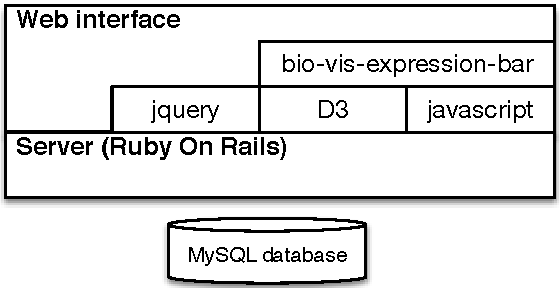
\includegraphics[width=0.8\textwidth]{expVIP/Figures/archDesign.pdf}
  \caption{General design of expVIP}
  \label{fig:poly:archDesign}
\end{figure}

\section{Database design} 
\label{exp:DB}

To address the different types of conditions over different experiments, expVIP is designed around a relational database. 
The design comprises two core groups of tables and two auxiliary tables that take care of different species and homoeologues (Figure \ref{fig:expvip:dbDesign}).


\begin{sidewaysfigure}
\centering
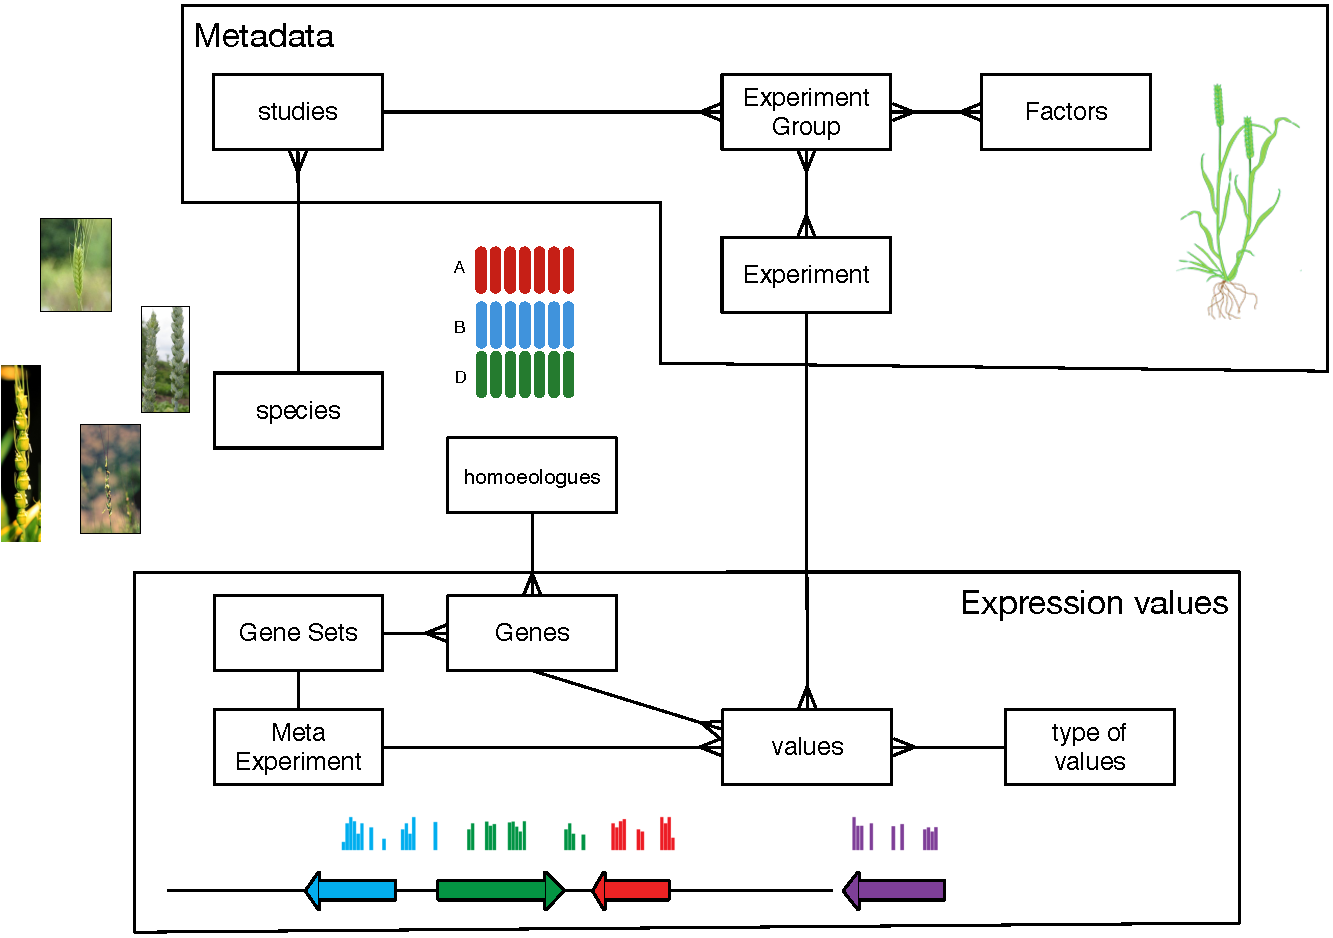
\includegraphics[width=0.85\textwidth]{expVIP/Figures/dbDesign.pdf}
\caption[expVIP database design]{Database design. The block on the top stores the meta-data about the experiments and the studies. The bottom block consist on the tables related to the expression values. Species and homoeologues are outside the main blocks as they are not core to the groups. The whiskers in the connections show the cardinality of the relationships.}
\label{fig:expvip:dbDesign}
\end{sidewaysfigure}

\begin{description}
\item[Metadata] The tables in this group contain the information of each one of the studies. 
\begin{description}
\item[Studies] holds general information for a study, which contain several experiments. The table also contains the reference to the paper where the data is published and the accession number for the study. 
\item[Experiment group] keeps together all the individual experiments that come from the same study and that were taken on the same condition (ie. replicates). 
\item[Factors] holds all the possible factors used to group the experiments. Each experiment group has many factors and each factor group has many experiment groups. As the experiment does not have a fixed number of columns representing each factor, it is possible to have any arbitrary number factors to group. 
\item[Experiment] holds the information of each individual experiment, with the corresponding accession. 
\end{description}
\item[Expression values.] The tables on this block contain the information for each genes and their expression values. 
\begin{description}
\item[Types of value] keeps a list of different units that are stored. On the original design \acrshort{tpm} and raw counts are set up, but as the units are not hard coded it is possible to use \acrshort{fpkm}, \acrshort{rpkm} or any other unit. 
\item[Gene Set] contains the name of a reference gene set for the analysis. On the original version of expVIP, the gene models from the \acrshort{iwgsc} as deposited in Ensembl release 26 were used \citep{Mayer2014}. However, this table allows to use several reference gene models on the same database. 
\item[Genes] are related to a \texttt{gene set}, so even if two genes coming from two different datasets share the same name it is possible to distinguish them and avoid ID collisions. This situation is unlikely to occur when using published references, but might arise when joining several \textit{de novo} gene model datasets. 
\item[Meta Experiment] allows to have the same data analysed with different tools. By default expVIP uses Kallisto \citep{Bray2016}. However other tools, or different versions of the same tool, can be used to repeat the analysis.   
\item[Values] have a domain that includes the \texttt{meta experiment}, \texttt{gene} and, \texttt{type of value}.
\end{description}
\item[Homoeologues] contains the relationship between genes. This allows to get the expression values of several related genes. 
\item[Species] contains the target species of a study. It is not linked to the gene models to allow the direct comparison between related species using the same gene models (ie, \texttt{T. aestivum} vs \texttt{T. turgidum}). 
\end{description}

In the cases where a relationship between tables is not unique, such as \texttt{experiment\_groups} having many \texttt{factors} and the \texttt{factors} having many \texttt{experiment\_groups}, storing of relationships is done with an auxiliary table (ie. \texttt{ExperimentGroups\_Factors}, not explicitly shown in Figure \ref{fig:expvip:dbDesign}, but implicit by the lines with whiskers). 

Once all the data is stored, the tables can be queried together to make clear the relationship between specific rows. 
One of the core tasks of expVIP is to get all the factors that define each experiment, in order to be able to merge similar studies. 
To retrieve the \texttt{experiments} and \texttt{factors} of an \texttt{experiment group}, the auxiliary tables \texttt{ExperimentGroups\_Factors}  and \texttt{experiment\_groups\_experiments} are used in the query. (Listing \ref{lst:exp:queryMetadata} and Table \ref{tab:exp:queryMetadata}).


\begin{code}[language=sql, caption={[Query experiments and factors]Query experiments and factorsQuery experiments and factors from accession 'DRR003148'},label=lst:exp:queryMetadata]
SELECT
	experiments.accession,  
	factors.factor,
	factors.description, 
	experiment_groups.name as expriment_group 
FROM factors 
JOIN ExperimentGroups_Factors 
	ON factors.id = ExperimentGroups_Factors.factor_id
JOIN experiment_groups 
	ON experiment_groups.id = ExperimentGroups_Factors.experiment_group_id
JOIN experiment_groups_experiments 
	ON experiment_groups_experiments.experiment_group_id = experiment_groups.id
JOIN experiments 
	ON experiments.id = experiment_groups_experiments.experiment_id
WHERE accession =  'DRR003148'
\end{code}

%\pagebreak
\begin{table}[h]
\caption[Results of query for metadata]{Results of querying the metadata for accession 'DRR003148' (Listing \ref{lst:exp:queryMetadata})}
\label{tab:exp:queryMetadata}
\begin{tabular}{llll}
\toprule
 accession   & factor                    & description    & expriment   \\
     &                     &     & group   \\
\midrule
 DRR003148   & Age                       & 24 days        & Group1            \\
 DRR003148   & High level age            & vegetative     & Group1            \\
 DRR003148   & High level stress-disease & no stress      & Group1            \\
 DRR003148   & High level tissue         & roots          & Group1            \\
 DRR003148   & High level variety        & Chinese Spring & Group1            \\
 DRR003148   & Stress-disease            & none           & Group1            \\
 DRR003148   & Tissue                    & roots          & Group1            \\
 DRR003148   & Variety                   & Chinese Spring & Group1            \\
\bottomrule
\end{tabular}

\end{table}

Likewise, to get the \texttt{expression\_values} for a \texttt{gene} with the corresponding unit (\texttt{type\_of\_values}) and \texttt{experiment} a simple query joining the four tables is used. 
The Listing \ref{lst:exp:queryExpValues} retrieves the \texttt{expression\_values} for the \texttt{gene} 'Traes\_5BS\_0AFC3F795.1', and the result is on Listing \ref{tab:exp:queryExpValues}

\begin{code}[language=sql, caption={[Query values for gene and experiment group] Query values from 'Group1' and gene 'Traes\_5BS\_0AFC3F795.1' },label=lst:exp:queryExpValues]
SELECT 
	genes.name as gene, 
	expression_values.value,
	experiments.accession,
	type_of_values.name as unit
FROM expression_values
JOIN genes 
	ON expression_values.gene_id = genes.id
JOIN type_of_values 
	ON type_of_values.id = expression_values.type_of_value_id
JOIN experiments 
	ON experiments.id = expression_values.experiment_id
WHERE 
	genes.name = 'Traes_5BS_0AFC3F795.1' 
\end{code}

\begin{table}[h]
\caption[Results of query for values]{Results of query to get the values for gene 'Traes\_5BS\_0AFC3F795.1' (Listing \ref{lst:exp:queryExpValues}), only 'Group1' is displayed from the output.}
\label{tab:exp:queryExpValues}
\begin{tabular}{lrlll}
\toprule
 gene                  &    value & accession   & experiment   & unit   \\
                    &     &    & group   &    \\
\midrule
 Traes\_5BS\_0AFC3F795.1 & 136.995  & DRR003148   & Group1             & count  \\
 Traes\_5BS\_0AFC3F795.1 & 120.683  & DRR003149   & Group1             & count  \\
 Traes\_5BS\_0AFC3F795.1 & 140.94   & DRR003150   & Group1             & count  \\
 Traes\_5BS\_0AFC3F795.1 &  24.2277 & DRR003148   & Group1             & tpm    \\
 Traes\_5BS\_0AFC3F795.1 &  23.9739 & DRR003149   & Group1             & tpm    \\
 Traes\_5BS\_0AFC3F795.1 &  24.9835 & DRR003150   & Group1             & tpm    \\
\bottomrule
\end{tabular}

\end{table}

With those two queries is enough to retrieve all the information required to do sub-groupings. 

The database is implemented using the \acrshort{rdbms} \texttt{MySQL 5.5}. 



\section{Data integration pipeline} 
\label{exp:pipeline}


To prepare the database, expVIP requires to have all the metadata for the experiments to integrate. 
ExpVIP contains tasks to load all the metadata and a wrapper for Kallisto that can be run from expVIP. 
Alternatively, the expression values can be calculated with another tool and loaded as a single file, this approach is preferred for a large set of samples (Figure \ref{fig:exp:loadPipeline}). 
Details on how to load the files in the database are in the expVIP tutorial (Appendix \ref{exp:tutorial}). 

\begin{figure}
\centering
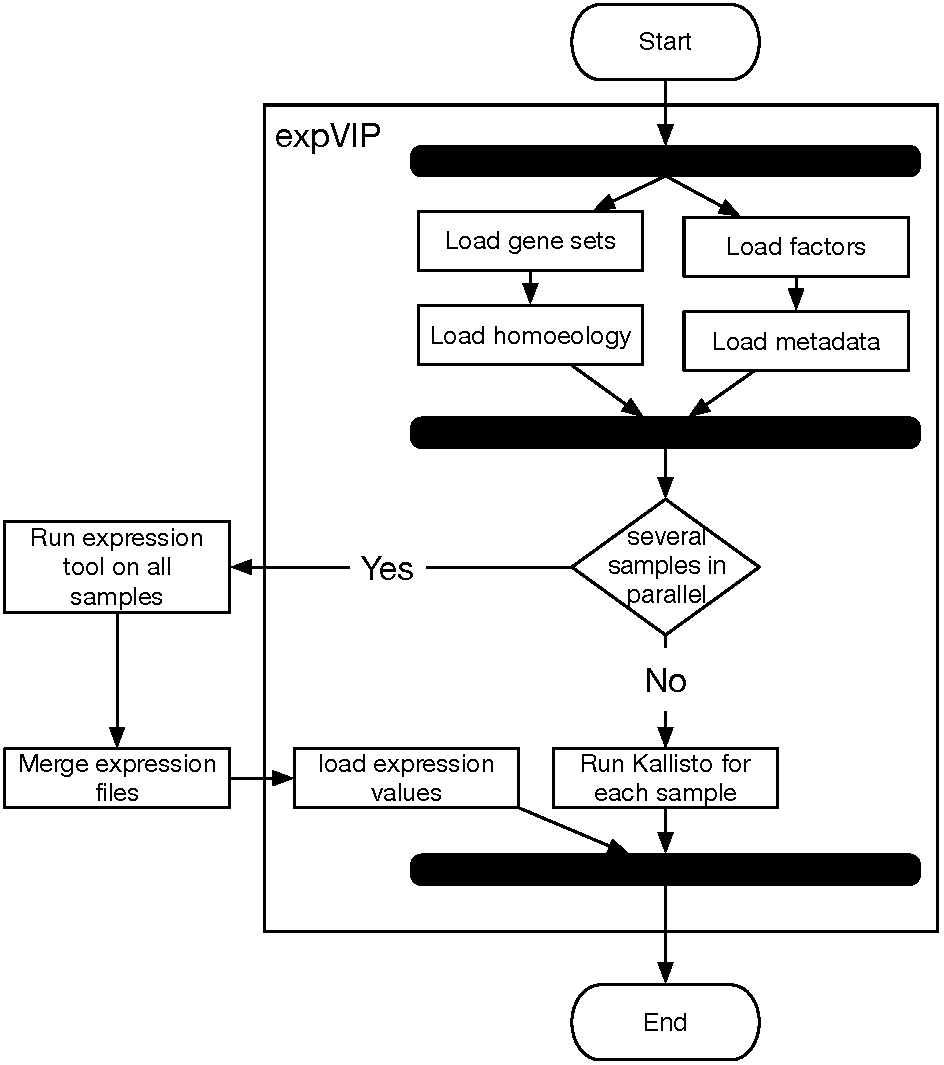
\includegraphics[width=1\textwidth]{expVIP/Figures/loadDataPipeline.pdf}
\caption[expVIP load data]{The pipeline for loading the data into expVIP. The black lines represent a border of tasks that are not required to be executed in a particular order.}
\label{fig:exp:loadPipeline}
\end{figure}

The required files for the metadata are:
\begin{description}
\item[Factors.] The file contains all the possible factors that can be used to group all the experiments. The file must contain the following columns (Table \ref{tab:exp:factors}):
\begin{description}
\item[factor] The category were the factor belongs. In the case of the initial dataset used in expVIP, the grouping factors are: Age, stress-disease, tissue and a corresponding 'High level' for each factor. The metadata file must contain a column corresponding to each one of this factors. 
\item[order] The default order in which to display each factor. This ensures that the age of the plants is sorted chronologically. 
\item[name] Long description of each level for the category. The values in this column must match the values in the metadata file (see below).
\item[short] Is a short name, used when the space to display the full description of the factor is not enough.
\end{description}
\begin{table}
\centering
\caption[Factors file]{Factors file. The table must be saved as a text file, with columns separated by tabs}
\label{tab:exp:factors}
\begin{tabular}{llll}
\toprule
factor & order & name & short \\
\midrule
Age & 1 & 7 days & 7d \\
Age & 2 & seedling stage & see \\
Age & 3 & 14 days & 14d \\
Age & 4 & three leaf stage & 3\_lea \\
Age & 5 & 24 days & 24d \\
High level age & 1 & seedling & see \\
High level age & 2 & vegetative & veg \\
High level age & 3 & reproductive & repr \\
High level stress-disease & 1 & none & none \\
High level stress-disease & 2 & disease & dis \\
High level stress-disease & 3 & abiotic & abio \\
High level stress-disease & 4 & transgenic & trans \\
High level tissue & 1 & spike & spike \\
High level tissue & 2 & grain & grain \\
... & & \\
\bottomrule
\end{tabular}
\end{table}
\item[metadata] The metadata file is the file that contains the information related to each study and the corresponding experiments. 
Each study contains several experiment groups (replicates), which in turn contain every individual experiment. 
The factors must be shared across experimental groups. 
\begin{description}
\item[secondary\_study\_accession] The accession number for experiments carried as part of a single study. This is usually the high level BioProject or SRA number. 
\item[run\_accession] The accession of the individual run. 
\item[scientific\_name] of the species. 
\item[experiment\_title] A description for the individual RNA-seq sample.
\item[study\_title] A description of the general study.
\item[Manuscript] The DOI of the study.
\item[Group\_for\_averaging] A description of the experiment. This must be the same all the replicates in the same study. 
\item[Group\_number\_for\_averaging] A short name for replicated experiments.  
\item[Total reads] (optional)
\item[Mapped reads] (optional)
\end{description}
Besides the main fields, each factor has a a corresponding column Variety, Tissue,Age, Stress-disease, High level variety, High level tissue, High level age and High level stress-disease

\item[Gene set] The gene set is provided as a single \verb|fasta| file. 
The file may contain alternative transcripts from the same gene. To identify this, the \verb|fasta| header may include the optional fields \texttt{gene} and \texttt{transcript}. 
In the absence of this, the only stored value is the name derived from the header, going from the \textgreater character to the first space on the line (Listing \ref{lst:poly:geneFa}). 

\begin{code}[label=lst:poly:geneFa, caption={[Gene set fasta file] A fasta entry on of the gene set.}]
>Traes_5BL_3FC5BA305.1 cdna:novel scaffold:IWGSC2:IWGSC_CSS_5BL_scaff_1082268:5:199:-1 gene:Traes_5BL_3FC5BA305 transcript:Traes_5BL_3FC5BA305.1
TGCTGCTGCTAGGCTTGAAGAGGTTGCTGGCAAGCTCCAGTCTGCTC
GGCAGCTCATTCAGAGGGGCTGTGAGGAGTGCCCCAAGAACGAGGAT
GTTTGGTTCGAGGCATGCCGGTTGGCTAGCCCAGATGAGTCAAAGGC
AGTAATTGCCAGGGGTGTGAAGGCAATTCCCAACTCTGTGAAGCTGT
GGCTGCA
\end{code}
\item[homoeologues] A file containing the homoeologues for the  A, B and D genomes. Currently these are the only supported default names. The file also includes a column with the gene name and to which Group (ie 1, 2, 3 ... 7) and Genome (ie A, B or D) it belongs (Table \ref{tab:exp:hom}).  

\begin{sidewaystable}
\centering
\caption[Homoeology file]{Example tabular file containing the homoeology across the three genomes. }
\label{tab:exp:hom}
\begin{tabular}{llllll}
\toprule
Gene & A & B & D & Group & Genome \\
\midrule
Traes\_5BS\_0AFC3F795 & Traes\_5BS\_0AFC3F795 & Traes\_5BS\_0AFC3F795 & Traes\_5DS\_C204EBAA9 & 5 & B \\
Traes\_5DS\_C204EBAA9 & Traes\_5DS\_C204EBAA9 & Traes\_5BS\_0AFC3F795 & Traes\_5DS\_C204EBAA9 & 5 & D \\
Traes\_7DL\_82360D4EE1 & Traes\_7DL\_82360D4EE1 & Traes\_7DL\_82360D4EE1 & & 7 & D \\
Traes\_2AL\_1368BE0AD & & Traes\_2AL\_1368BE0AD & Traes\_2BL\_CD459994C1 & 2 & A \\
... & & & & &  \\
\bottomrule 
\end{tabular}
\end{sidewaystable}
\end{description} 

expVIP includes several tasks to load the different files. 
For example, to load the factors the \verb|load_data:factor| starts a transaction (Listing \ref{lst:exp:loadFactor}; line 2) to ensure that all the data is loaded, and if for some reason the load fails, the database is restored to the previous status.
In the transaction, the file is read row by row using the \verb|csv| library (line 3).
The function \verb|find_or_create_by| is a function that \acrshort{ror} provides on models to create an entry in the table, or update it if already exists.
Each row is used to create or update a \verb|Factor| (lines 374-376). 
A similar strategy is used for all the files that are regular tables. 

\begin{code}[label=lst:exp:loadFactor, language=ruby, caption={[Load factors]Task that loads factors}]
task :factor, [:filename] => :environment do |t, args|
  ActiveRecord::Base.transaction do 
    CSV.foreach(args[:filename], :headers => true, :col_sep => "\t") do |row|
      factor = Factor.find_or_create_by(:factor=>row["factor"],  :description=>row["name"],  :name=>row["short"])
      factor.order = row["order"].to_i
      factor.save!
    end
  end
end
\end{code}

The gene sets are loaded slightly differently, as the input is a \verb|fasta| file, as opposed to tabular file. 
The reader for the \verb|FastaFormat| from BioRuby \citep{Goto2010} is used to read the file (Listing \ref{lst:exp:loadGenes}; line 4). 
Since expVIP only records the name of the genes, only the id of the fasta sequence is extracted (lines 6-79). 
The name is stored in the name and cDNA columns. 
The parser for entries from ensembl, such the one in Listing \ref{lst:poly:geneFa} include code to load the \acrshort{cdna} and transcript fields correctly. 

\begin{code}[language=ruby, caption={[Load genes from Fasta]Task that load genes from a fasta file}, label=lst:exp:loadGenes]
task :de_novo_genes, [:gene_set,:filename] => :environment do |t, args|
  ActiveRecord::Base.transaction do
    gene_set = GeneSet.find_or_create_by(:name=>args[:gene_set])
    Bio::FlatFile.open(Bio::FastaFormat, args[:filename]) do |ff|
      ff.each do |entry| 
        arr = entry.definition.split(/\s+/)
        name = arr[0]
        g = Gene.new 
        g.gene_set = gene_set
        g.name = name
        g.cdna = name
        g.save!
      end
    end
  end
end
\end{code}

There are two options to load the expression values from the database: a matrix with all the expression values and running \verb|Kallisto| from expVIP. 

The task in Listing \ref{lst:exp:loadValues} loads the expression values from a tabular file with the genes as rows and the values as columns. 
The exception handling and messages are removed 
The task requires the following arguments:

\begin{description}
\item[\texttt{meta\_experiment}.] A name for the analysis. This can be the name of the tool used for the expression quantification combined with the name of the reference, as a single text variable. 
\item[\texttt{gene\_set}.] The reference used for the analysis. 
\item[\texttt{value\_type}.] The unit of the file (ie.  \acrshort{tpm}, count)
\item[\texttt{filename}.] The file that is going to be loaded in the database. 
\end{description}

The steps to load the values are:
\begin{enumerate}
\item A transaction is initiated at the beginning of the task, to ensure that if any step fails and the execution is aborted the database will stay in a consistent state (Listing \ref{lst:exp:loadValues}; line 2).
\item The connection is assigned to the variable \verb|conn|, to be able to execute queries directly to the database (line 3).   
\item The \verb|meta_experimet|, \verb|gene_set| and \verb|value_type| are loaded and stored to get the corresponding IDs in the insertion (line 4).
\item All the \verb|Genes| and \verb|Experiments| are loaded in their corresponding hash table, to be able to get the IDs when the actual values are inserted (lines 7-11). 
\item The file is read with the \verb|CSV| library from Ruby, keeping the headers to be able to assign the correct experiment (line 14). 
\item The first column is named \verb|target_id| and contains the gene name. The ID of the gene  in the database is retrieved from the previously loaded hash (lines 15-16)
\item Each column is iterated and the values needed to execute the insertion to the database are concatenated. 
\item Whenever the number of queued insertions reaches 1,000, the command to perform the insertions is executed (line 25). 
\item As the number of genes is not usually a multiple of 1,000, when the process finished reading the file an extra insertion is executed to empty the queue (line 30).
\end{enumerate}

The decision to execute the insertions in batches of 1,000 objects is to reduce the number of processes running in the database, while keeping low the memory usage of the application. 
This approach is faster than using the functions for insertions \acrshort{ror} on multiple values. 
For trivial operations, the functions from the framework are used, as they are easier to maintain (compare insertion in line 4 to the block of code from line 18 to 26). 

\begin{code}[language=ruby, label=lst:exp:loadValues, caption={[Load expression values from file] Task to load the expression values from a tabular file.}]
task :values, [:meta_experiment, :gene_set, :value_type, :filename ] => :environment do |t, args| 
ActiveRecord::Base::transaction do
conn = ActiveRecord::Base.connection
meta_exp = MetaExperiment.find_or_create_by(:name=>args[:meta_experiment])
gene_set = GeneSet.find_by(:name=>args[:gene_set])
value_type = TypeOfValue.find_or_create_by(:name=>args[:value_type])
experiments = Hash.new
meta_exp.gene_set = gene_set
genes = Hash.new
Gene.find_by_sql("SELECT * FROM genes where gene_set_id='#{gene_set.id}'").each {|g| { genes[g.name] = g.id}
Experiment.find_each{|e| experiments[e.accession] = e.id}
count = 0
inserts = Array.new
CSV.foreach(args[:filename], :headers => true, :col_sep => "\t") do |row|
	gene_name = row["target_id"]
	gene = genes[gene_name]
	row.delete("target_id")
	row.to_hash.each_pair do |name, val| 
		val = val.to_f 
		str = "(#{experiments[name]},#{gene},#{meta_exp.id},#{value_type.id},#{val},NOW(),NOW())"
		inserts.push str          
	end
	count += 1
	if count % 1000 == 0 
		sql = "INSERT INTO expression_values (`experiment_id`,`gene_id`, `meta_experiment_id`, `type_of_value_id`, `value`,`created_at`, `updated_at`) VALUES #{inserts.join(", ")}"
		conn.execute sql
		inserts = Array.new
	end
end
sql = "INSERT INTO expression_values (`experiment_id`,`gene_id`, `meta_experiment_id`, `type_of_value_id`, `value`,`created_at`, `updated_at`) VALUES #{inserts.join(", ")}"
conn.execute sql
end
end
\end{code}


\begin{wrapfigure}{R}{0.45\textwidth}
\centering
%\rule{3cm}{7cm}
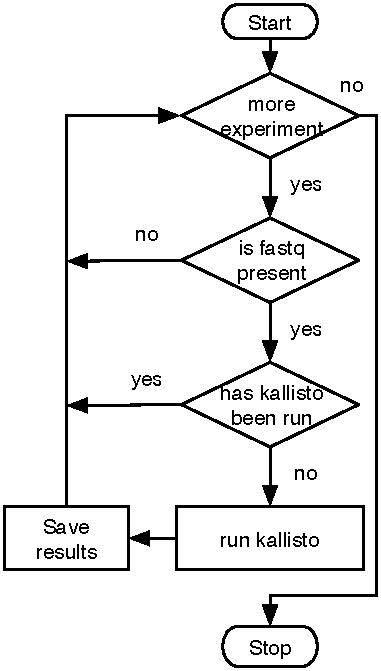
\includegraphics[width=0.45\textwidth]{LitReview/Figures/runKallisto.pdf}
\caption  {Steps to run and load Kallisto}
\label{fig:exp:runKallisto}
\end{wrapfigure}

Alternatively, expVIP can execute \verb|Kallisto| on all the samples loaded in the database. 
For this purpose, expVIP stores the raw reads in FastQ format, organized in directories named with the same accessions as in the metadata (ie a directory named \verb|DRR003148| contains the reads for the metadata displayed in table \ref{tab:exp:queryMetadata}). 
expVIP takes all the accessions for the experiments in the database and searches for the corresponding folder. 
If the folder exists and if it contains the \verb|fastq| files, then it is deemed as valid. 
If the folder already has the \verb|kallisto| output, the next folder is evaluated, otherwise \verb|kallisto| is executed with its default settings and the results are loaded into the database. 
This process is repeated for all the accessions (Figure \ref{fig:exp:runKallisto}).  
This pipeline allows to populate the database partially, in case that not all the experiments are ready from the beginning. 

New experiments can be added to the existing metadata file  or to a new file; the expVIP loading procedure then can be run again to update the list of experiments and the corresponding expression values. 
This design allows to keep the database updated as more experiments become available. 
The fact that the loading is done in transactions ensures that the database is kept consistent, regardless of potential errors in the input files. 

\section{Graphical interface}
\label{exp:gui}  
%How the expression can be displayed filtered, and sorted
With the expression across experiments integrated in a single database, the next challenge is to make the data accessible to a wide audience. 
\acrshort{ror} has tasks to automate the construction of controllers and views from the \acrshort{mvc} metaphor, helping on the retrieval and formatting of the raw data. 
However, the main objective was to visualise the data from all the experiments as intuitively as possible. 
To make the visualisation dynamic in a browser, the use of \verb|JavaScript| is necessary, as it is the only widely adopted programming language used for web content. 
Among the tools built on the top of \verb|JavaScript|, \verb|D3| is a framework designed explicitly to do dynamic visualisations \citep{Bostock2011}. 

Usability was a top priority on the design of the visualisation component for expVIP. 
The time needed to learn, performance are accuracy were taken into account when designing expVIP. 
As memorability and satisfaction are subjective, they were not directly tested for during development.  


\begin{description}
\item[Time to learn.] The controls are located in two blocks, one for global controls (ie. unit, save plot) and one to modify the factors, close to the factor they affect (Figure \ref{fig:exp:layout}). 
\item[Performance.] All the data for the genes being displayed is loaded from the database in a single transaction. The data is available in the cache of web browser and whenever the user changes anything in the visualisation, new values are calculated locally. 
\item[Accuracy.] As knowing what the users will do is not obvious, the visualisation was given to a panel of potential users (other members of the Uauy lab) for comments. In previous versions the legends were a confusing and the location of the buttons was too distant from the aspect of visualisation that they controlled. After reviewing the feedback, the accuracy was improved.  Also, the position of the controls don't change, regardless of the representation of the data (bar plot or heatmap). 
\end{description}

\begin{figure}
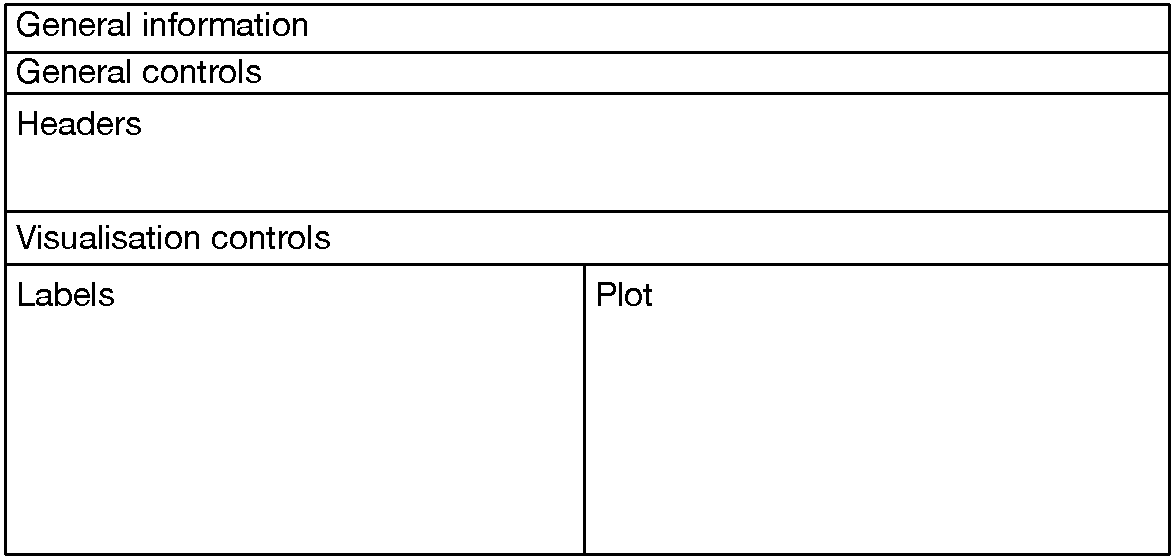
\includegraphics[width=1\textwidth]{expVIP/Figures/UIsketch.pdf}
\caption[expVIP \acrshort{gui} layout]{expVIP \acrlong{gui} components components. The top bar shows a short description of what is displayed. The General and Visualisation controls contain the buttons and menus that enable the interaction with the figure. The Headers, Labels and Plot are the actual components of the visualisation}
\label{fig:exp:layout}
\end{figure}

The elements in the graphical are shown in Figures \ref{fig:exp:tutorial1}, \ref{fig:exp:tutorial2} and \ref{fig:exp:tutorial3}, with a description of each element of the \acrshort{gui} listed below. 

\begin{figure}
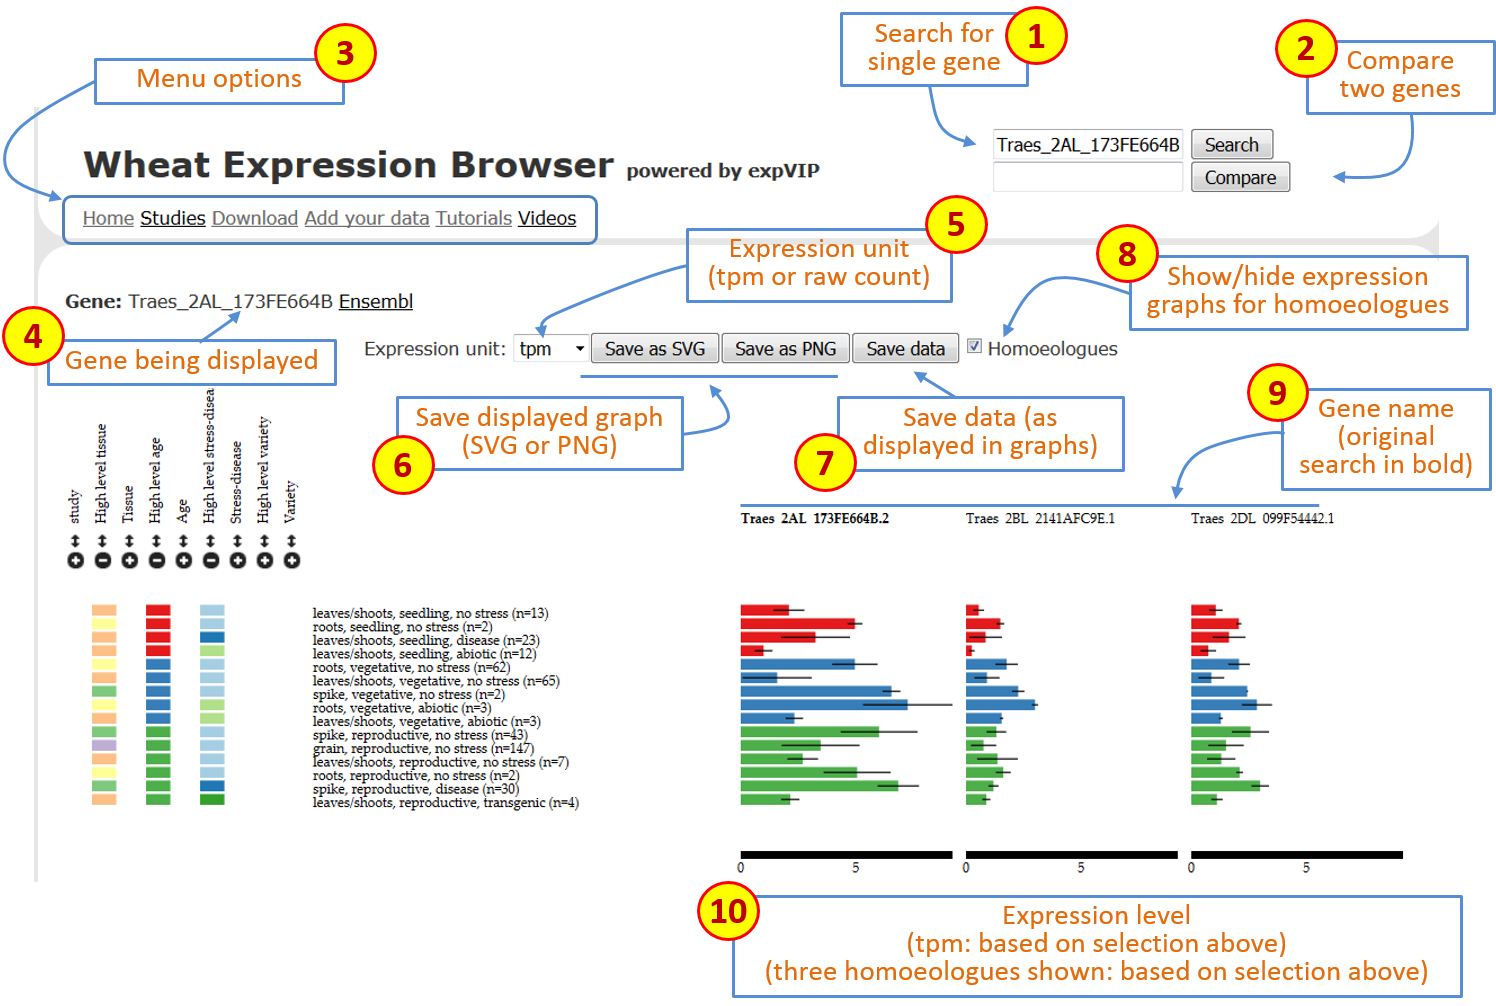
\includegraphics[width=1\textwidth]{expVIP/tutorial/images/Figure1.png} 
\caption{Features on expVIP}
\label{fig:exp:tutorial1}
\end{figure}
\begin{enumerate}
\item
  \textbf{\lstinline!Search box!}: at any point it is possible to type a new gene name (based on Ensembl Plants nomenclature) and generate a new set of expression data.
\item
  \textbf{\lstinline!Compare box!}: it is possible to add a second gene and press the \lstinline!Compare! button to generate two expression graphs drawn at the same scale.
\item
  \textbf{\lstinline!Menu options!}: has several links on the details of the study and tutorial. The menu can be edited to customize instances of expVIP. 
\item
  \textbf{\lstinline!Gene!}: shows the currently displayed gene, with a link to Ensembl to the corresponding description. 
\item
  \textbf{\lstinline!Expression unit!}: selects the expression unit to visualise. This can be either \gls{tpm} or  estimated counts. If other units are loaded in the database, they will appear in this field. 
\item
  \textbf{\lstinline!Save graph!}: these two buttons allow users to save the current graphs in either \lstinline!SVG! (to work on Adobe Illustrator) or as \lstinline!PNG! files. 
  The export process selects the graphical elements from the visualization and binds them together on a single \verb|SVG| file. The reasons to follow this process are: to ensure that the plot reflects the user selection; remove the elements that do not have a meaning in a static context and; allow the user to format the image with publication quality (Figure \ref{fig:exp:exportImage}).

\begin{figure}

\begin{subfigure}{1\textwidth}
\caption{}
\label{fig:exp:exportLayout}
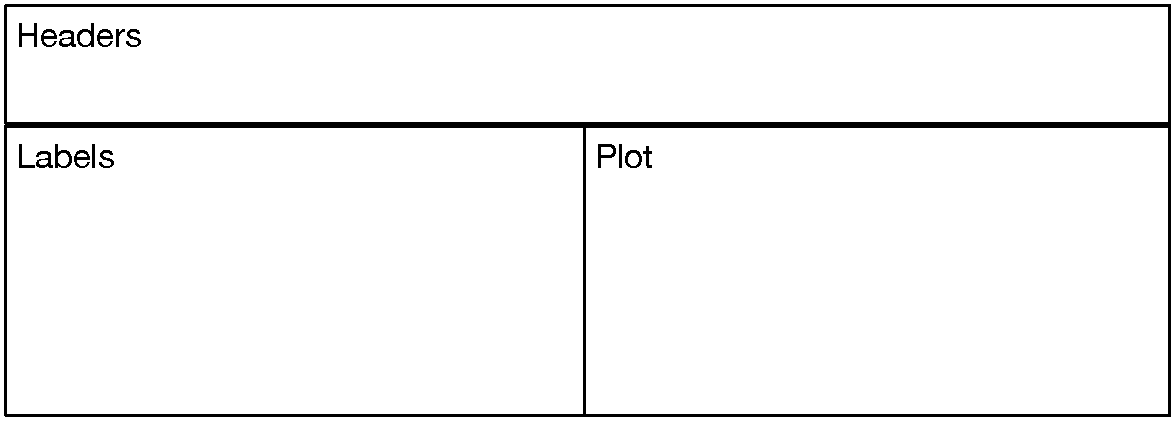
\includegraphics[width=1\textwidth]{expVIP/Figures/Exportsketch.pdf}
\end{subfigure}

\begin{subfigure}{1\textwidth}
\caption{}
\label{fig:exp:exportImageSample}
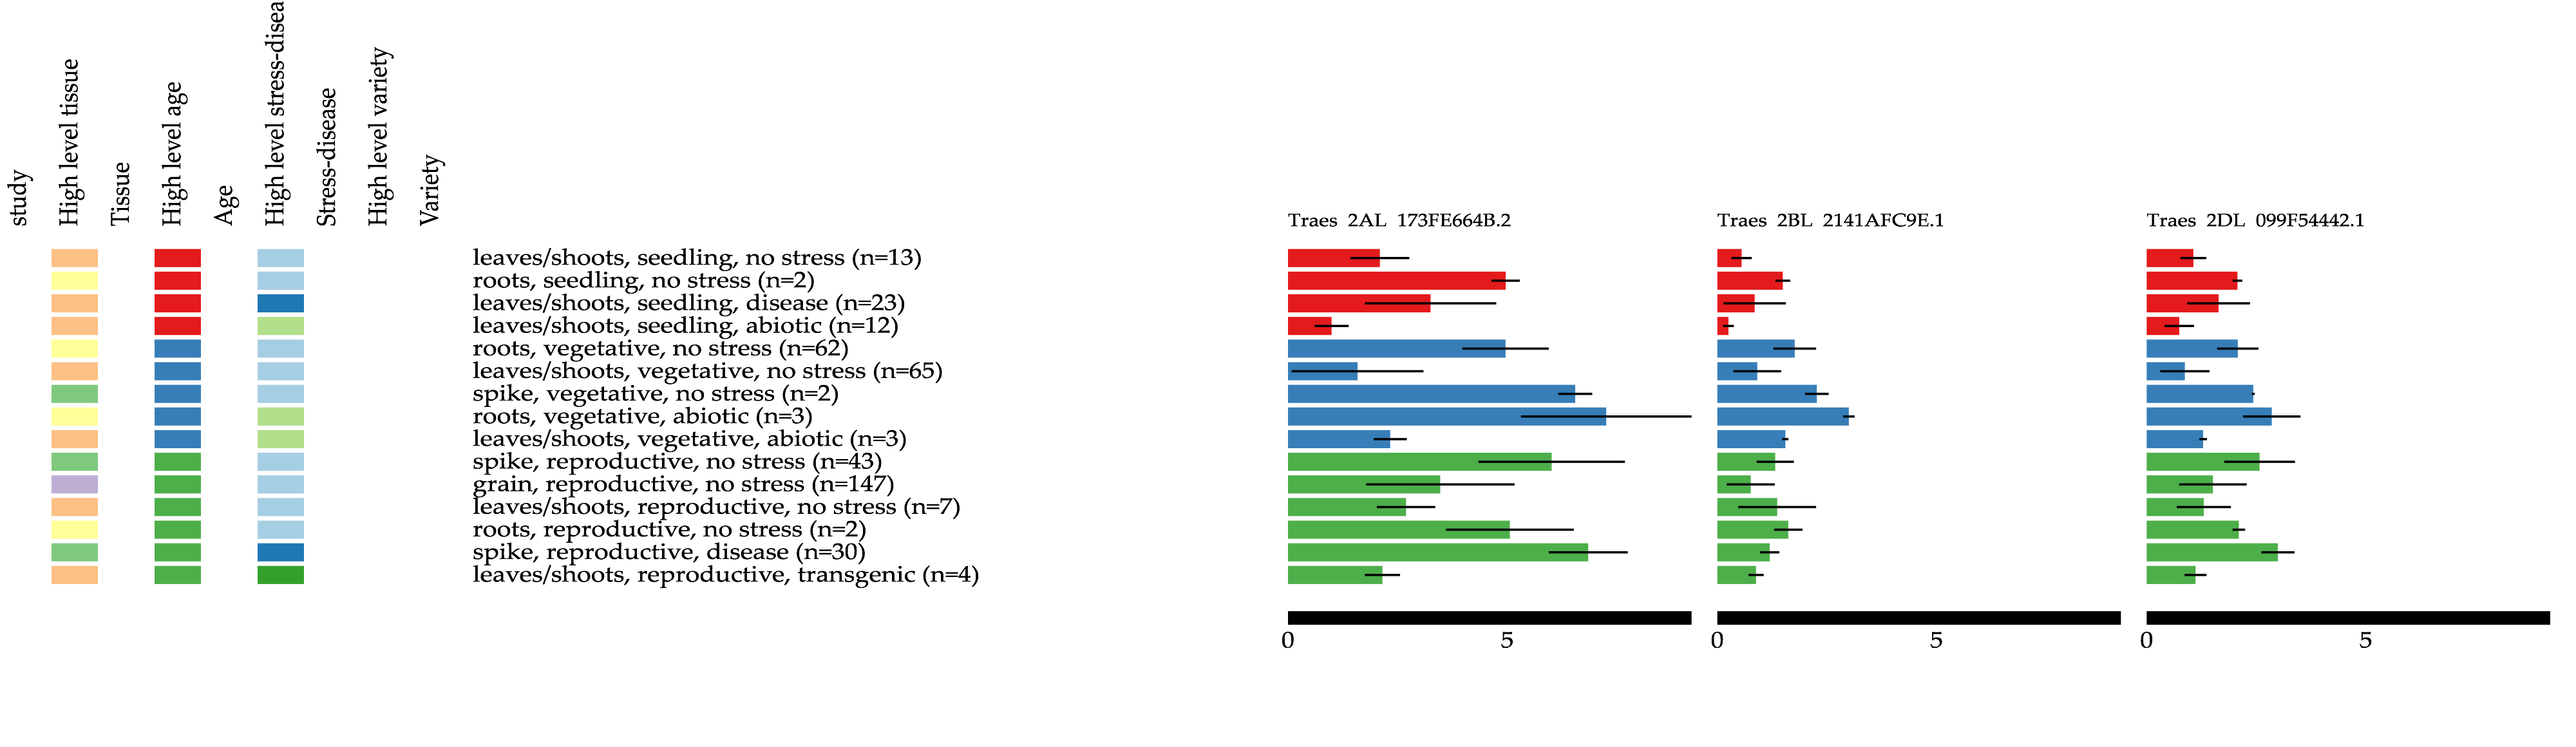
\includegraphics[width=1\textwidth]{expVIP/Figures/tutorialSampleOutput.png}
\end{subfigure}

\caption[expVIP export image]{expVIP export image. (\ref{fig:exp:exportLayout}) \acrshort{gui} components components exported in image} (\ref{fig:exp:exportImageSample}) The exported components from Figure \ref{fig:exp:tutorial1}) 
\label{fig:exp:exportImage}.
\end{figure}

\item
  \textbf{\lstinline!Save data!}: downloads a \lstinline!csv! file with the data with the current selection and
  order of factors as displayed on the screen. The data will include the standard errors and the number of samples that make up each value. 
  An example of how the output looks is in Listing \ref{lst:exp:exportSample}. 


\item
  \textbf{\lstinline!Homoeologues!}: this button displays the
 graphs of known homoeologues of the original primary gene. This gene is highlighted in bold and the homoeologous graphs will be displayed according to A, B, D genome ordering. 
 The scale of all the homoeologues is the same to facilitate the comparison between them. 
\item
  \textbf{\lstinline!Gene names!}: each displayed gene is labelled on this block.  
  If the list of genes is too long, the gene names are rotated for readability. 
  In case that a gene name is too long to fit, the font is scaled to the largest size that will fit in the designated area. 
\item
  \textbf{\lstinline!Expression level!}: the expression level adjusts according to the expression of each set of gene homoeologues. The scale remains consistent across homoeologues to allow comparison. 
  The values are based on the unit selected in the \lstinline!expression unit! box (see point 5 above).

\begin{figure}
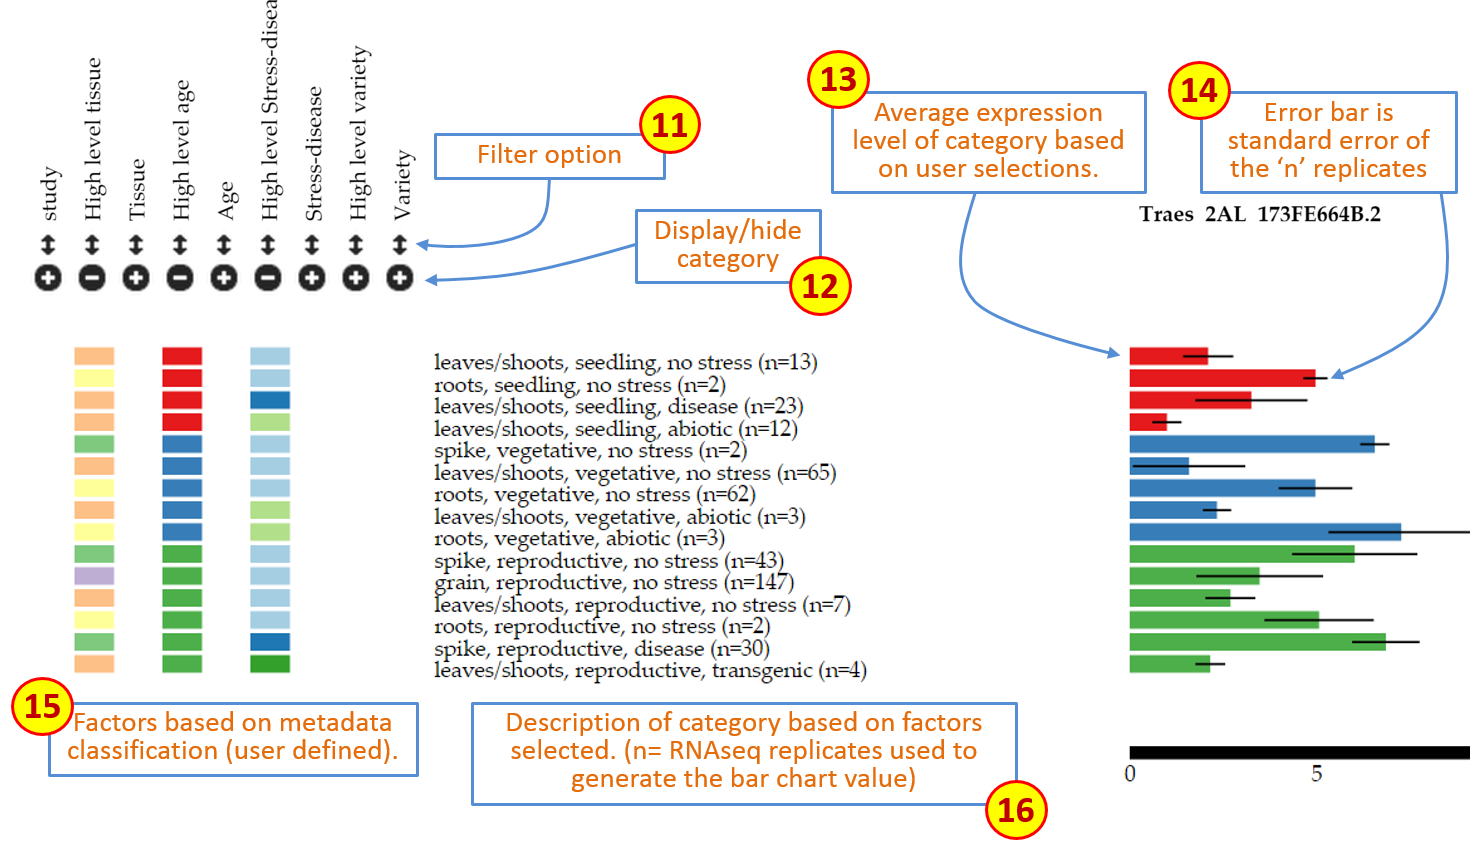
\includegraphics[width=1\textwidth]{expVIP/tutorial/images/Figure2.png} 
\caption{Features on expVIP (continued)}
\label{fig:exp:tutorial2}
\end{figure}

\item
  \textbf{\lstinline!Filter!}: opens a pop-up window revealing the levels of the selected category. 
  By default, all the levels are selected, but the users can decide to exclude from the visualisation experiments containing any level. 
  The order of the levels can be modified by dragging the levels on the the pop-up window. 
\item
  \textbf{\lstinline!Display/hide category!}: Each category
  can be displayed or hidden by pressing the \lstinline!+/-! button.
  As categories are added or removed the expression graphs show the new values for the new groups. 
  Data is not removed when changing the displayed categories, instead the values are distributed according to the new groups (the number of samples remains the same). 
  The colours below the category correspond to each level, and the plot is coloured according to the sorting category. 
\item
  \textbf{\lstinline!Expression bars!}: These bars represent the expression level for the \verb|n| grouped samples according to
  the chosen categories (11 and 12 above).
  When hovering over the bar with the mouse a small tooltip will appear, containing the expression level (\lstinline!tpm! or \lstinline!counts!) and the standard error (sem) used for the error bars (see 14)
\item
  \textbf{\lstinline!Error bars!}: Standard error of the means for the \verb|n| expression values on which the bar graph is based.
\item
  \textbf{\lstinline!Factors!}: The colour of the rectangles represents the displayed categories, according to the selection criteria (11 and 12 above). 
  To clarify the meaning of the colour, hovering above the rectangle displays a tooltip with the long name of the examined level. 
\item
  \textbf{\lstinline!Description!}: Textual description of the grouped factors, according to the selection criteria (11 and 12 above). 
  The number of grouped samples is also displayed.

\begin{figure}
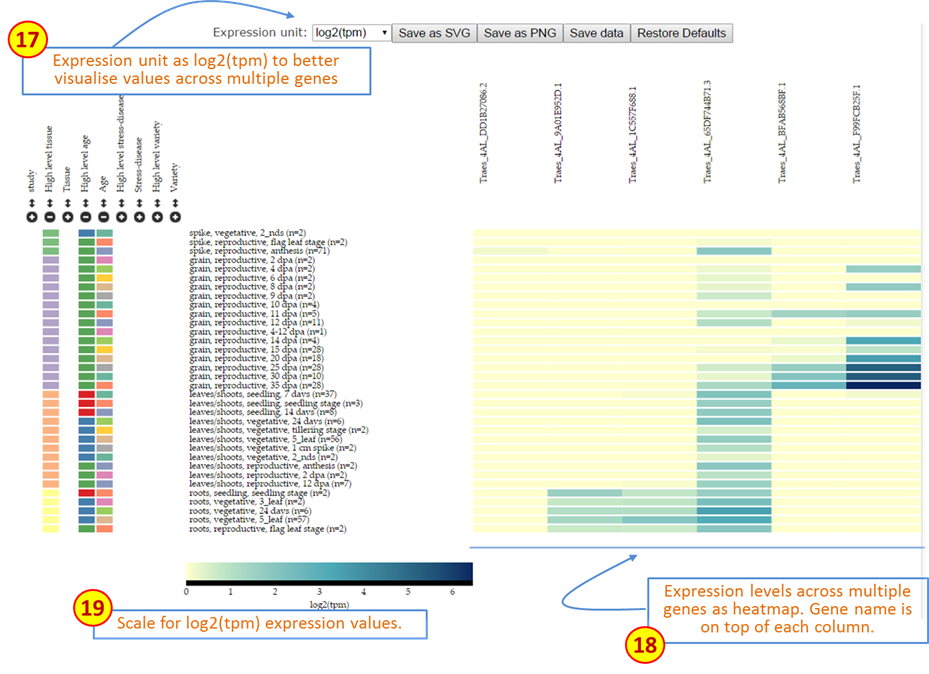
\includegraphics[width=1\textwidth]{expVIP/tutorial/images/Figure2a.png} 
\caption{Features on expVIP for Multiple gene comparisons}
\label{fig:exp:tutorial3}
\end{figure}

\item
  \textbf{\lstinline!Expression unit!}: For heatmaps, the default unit log2(tpm) as the logarithmic scale provides a better context for comparisons acorss several genes.
\item
  \textbf{\lstinline!Heatmap!}: To compare several genes, the values are represented as a heatmap. The sorting and filtering is done with the same controls as for single genes.
  Up to 50 genes are displayed in the heatmap, as more genes will degrade the performance of the database, and the visual clutter makes the plot hard to interpret. 
  This view allows to visualise several candidate genes for a trait expressed under certain conditions and quickly asses which one is a good candidate for further research. 
\item
  \textbf{\lstinline!Scale!}: The scale is calculated according to the highest displayed value in the current heatmap. 
  Since logarithmic values below 1 result in negative values and anything with a \acrshort{tpm} under 2 is considered as very low expressed, every value lower than 1 is plotted as 0.
\end{enumerate}
For a comprehensive user manual see Appendix \ref{exp:tutorial}. 

%%\section{Virtual Machine}
%%\label{exp:vm}
\unsure{If I have time, I'll add the section about the virtual machine, as I would also need to add something in the background on virtualisation, it can potentially be a sink of time}

\begin{landscape}
\begin{code_2}[label=lst:exp:exportSample, caption={[Export data example] Export data example, corresponding to the data plot in Figure \ref{fig:exp:tutorial1}}]
High level age	seedling, vegetative, reproductive, 
High level stress-disease	no stress, disease, abiotic, transgenic, 
High level tissue	spike, grain, leaves/shoots, roots, 
High level variety	Chinese Spring, other, Nullitetra Chinese Spring, 
	tpm	SEM	tpm	SEM	tpm	SEM	
	Traes_2AL_173FE664B.2	Traes_2AL_173FE664B.2	Traes_2BL_2141AFC9E.1	Traes_2BL_2141AFC9E.1	Traes_2DL_099F54442.1	Traes_2DL_099F54442.1	
roots, vegetative, no stress(n=62)	4.96	0.99	1.77	0.49	2.08	0.47
roots, vegetative, abiotic(n=3)	7.26	1.95	3.00	0.13	2.85	0.66
leaves/shoots, vegetative, no stress(n=65)	1.59	1.50	0.91	0.55	0.87	0.56
leaves/shoots, vegetative, abiotic(n=3)	2.33	0.38	1.55	0.07	1.29	0.09
spike, reproductive, disease(n=30)	6.85	0.90	1.19	0.22	2.99	0.38
spike, reproductive, no stress(n=43)	6.01	1.67	1.32	0.43	2.58	0.81
grain, reproductive, no stress(n=147)	3.47	1.69	0.76	0.55	1.51	0.77
leaves/shoots, reproductive, transgenic(n=4)	2.15	0.40	0.88	0.18	1.11	0.25
leaves/shoots, reproductive, no stress(n=7)	2.69	0.67	1.37	0.89	1.30	0.62
leaves/shoots, seedling, disease(n=23)	3.25	1.50	0.85	0.71	1.64	0.72
leaves/shoots, seedling, no stress(n=13)	2.10	0.67	0.55	0.23	1.07	0.29
leaves/shoots, seedling, abiotic(n=12)	0.99	0.39	0.25	0.12	0.74	0.34
roots, seedling, no stress(n=2)	4.96	0.32	1.49	0.17	2.07	0.11
roots, reproductive, no stress(n=2)	5.06	1.46	1.62	0.32	2.10	0.14
spike, vegetative, no stress(n=2)	6.55	0.39	2.27	0.27	2.43	0.03
\end{code_2}
\end{landscape}

\section{Discussion.} 


%The use of previously published studies is a valuable resource. 

In model organisms there are several on-line resources that aggregate the raw data and meta analysis of several studies. 
For example, the Expression Atlas \acrshort{ebi}  includes over 2,000 studies for \textit{Arabidopsis thaliana} inclusive of other technologies besides RNA-Seq (ie Affymetrix expression arrays). 
However, when I started the development of expVIP the Expression Atlas only included a couple of baseline experiments and WheatExp had not been published yet (Figure \ref{fig:exp:timeline}).  

\begin{figure}
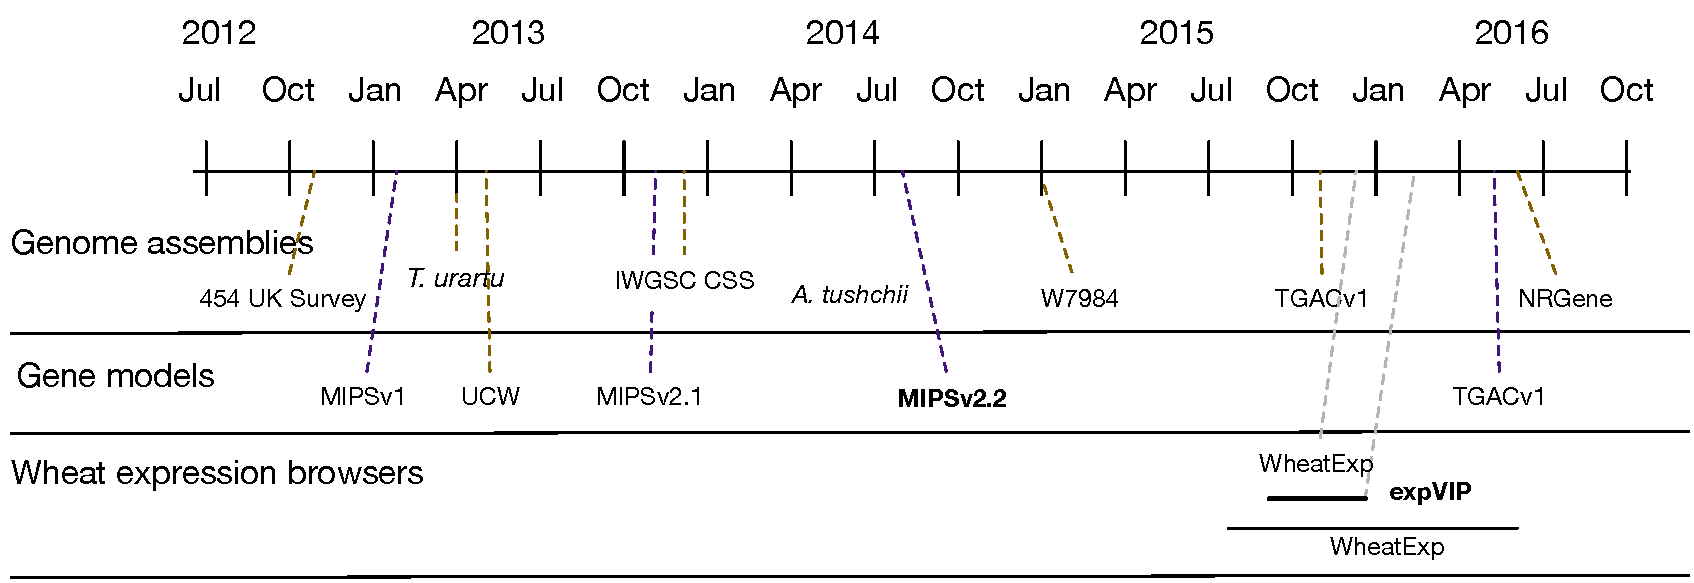
\includegraphics[width=1\textwidth]{expVIP/Figures/Timeline.pdf}
\caption[expVIP resources time line]{expVIP resources time line. In bold the line of the time for development of expVIP and the annotation used. The Expression Atlas has a line starting on the initial study deposited on it till the last update, as of September 2016.}
\label{fig:exp:timeline}
\end{figure}

%When I started the development of expVIP none of the expression browsers mentioned in Section \ref{exp:alternative} had data for wheat. 


WheatExp was developed roughly at the same time of expVIP and contains 6 studies (against 16 on expVIP; \citealt{Pearce2015b}). 
Four of the studies in WheatExp are on hexaploid wheat and are included in expVIP as well. 
In WheatExp, the expression for each gene is displayed on the context of the original experiment without a direct comparison between studies. 
However, because the studies are kept independently the levels of the categories are a direct reflection of the original studies. 
%\unsure{Why is this fact a detriment for WheatEXP?}
WheatExp allows to search genes by sequence, a feature not implemented in expVIP. 

The Expression Atlas from \acrshort{ebi}, as of September 2016, contains 10 studies, 4 baseline and 6 for differential expression \citep{Petryszak2016}. 
ExpVIP contains studies released before \acrshort{ebi} started to upload expression experiments for wheat. 
Even if some of the most recent studies in the Expression Atlas are not included in expVIP yet, we are in the process of updating our tool to include studies published after the initial release.
In terms of visualisation, the \acrshort{ebi} included a heatmap to compare to different factors at the same time for given gene (ie. tissue vs stress); the same information can be displayed on expVIP by sorting by two factors.


Most of the RNA-Seq studies report their results in terms of \acrshort{rpkm}. 
This normalisation, which is computed for done for each feature $g$ in the reference $G$, requires the count of the number of reads  $r_{g}$, the feature length $\textrm{fl}_{g}$ and the total number of mapped reads $R$ (Figure \ref{fig:exp:units}; equations \ref{eq:exp:R} and  \ref{eq:exp:rpkm} \citealt{Mortazavi2008}).
As the denominator of \ref{eq:exp:rpkm} is based on the number of mapped reads rather than the number of nucleotides covered, RPKM does not allow to compare correctly results obtained between different samples, or even results from the same sample when the average read length changes due to variations in the experimental protocol \citealt{Wagner2012}.
%\unsure{The original sentence was not completely clear; I hope this version elucidates more}

\begin{figure}
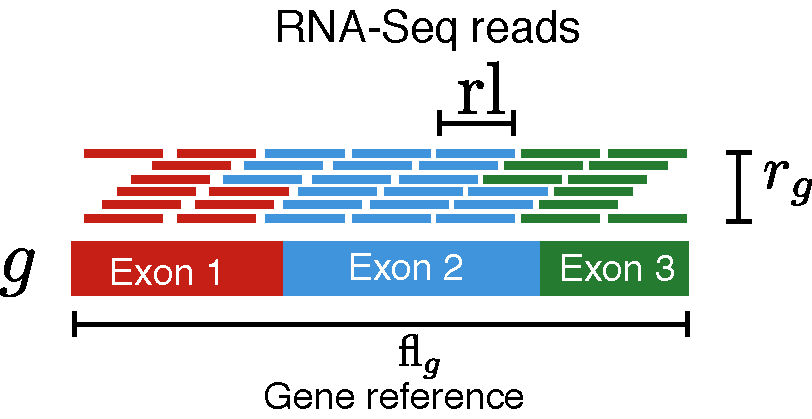
\includegraphics[width=1\textwidth]{expVIP/Figures/Units.pdf}
\caption[Units used for expression normalisation]{Units used for expression normalisation}
\label{fig:exp:units}
\end{figure} 


\begin{equation}
\label{eq:exp:R}
R = \displaystyle\sum_{g \in G} r_{g} 
\end{equation}

\begin{equation}
\label{eq:exp:rpkm}
  \textrm{RPKM}_{g} = \frac{r_{g}\times10^9}{\textrm{fl}_{g}\times R}
\end{equation}

The \acrshort{tpm} is an alternative to \acrshort{rpkm} that approximates the total number of transcripts $T$ as a normalisation factor (equation \ref{eq:exp:T}). 
Besides the previously described parameters, the \acrshort{tpm} also includes the read length $\textrm{rl}$, which is dependent on the study. 
This formula assumes that each read corresponds to a full observed transcript (equation \ref{eq:exp:tpm}; \citealt{Wagner2012}). 
%\unsure{Do you mean here that the formula assumes that each read has been assigned *unambiguously* to a single transcript? The sentence is unclear.}

\begin{equation}
\label{eq:exp:T}
T = \displaystyle\sum_{g \in G} \frac{r_{g} \times \textrm{rl}}{\textrm{fl}_{g}}
\end{equation}

\begin{equation}
\label{eq:exp:tpm}
  \textrm{TPM}_{g} = \frac{r_{g} \times \textrm{rl}\times10^6}{\textrm{fl}_{g} \times T }
\end{equation}


One of the aims in developing TPM was to be able to compare samples from different studies; as it is more stable across different experiments, we decided to use it as the main unit of comparison in expVIP. 
After we took the decision of which unit to use, we found a couple of tools, Kallisto \citep{Bray2016} and Sailfish \citep{Patro2014}, that could calculate the TPMs directly from mapping the reads to a reference, without producing a precise alignment.
The main advantage of only doing mapping, without aligning is a significant reduction in both the computational resources and the time needed to analyse a sample.

%\unsure{These lists would really benefit from being multi-line, not all inline like they are displayed at the moment.}
The traditional pipeline to quantify expression from RNA-Seq consists on the following steps:
\begin{enumerate}
  \item Index the reference. Only done once, as the same index can be used for all the samples. 
  \item Align the reads to the reference. 
  \item Sort the alignment and remove duplicates. 
  \item Quantify the expression.  
\end{enumerate}
This is the prevailing pipeline for expression analysis. 
In my experience, on a computing cluster it takes between 6 to 8 hours to process each wheat sample on a computing cluster, using multiprocessing and up to 24 Gb of RAM (Figure \ref{fig:exp:alnPipeline}). 
This pipeline is usually implemented by aligning the reads with \verb|BWA| \citep{Li2009} or \verb|tophat|  \citep{Trapnell2012} and the quantification is performed with tools like \verb|HTSeq| \citep{Anders2015} or \verb|cufflinks| \citep{Trapnell2012}.

%\unsure{Again, this list would be clearer as one item per line rather than inline.}
An advantage of using a mapper is that the quantification pipeline is shorter:
\begin{enumerate}
  \item Index the reference. Only done once, as the same index can be used for all the samples. 
  \item Map the reads to the reference and quantify the expression in a single program.   
\end{enumerate}
Since mapping does not require the precise alignment of every single base on the read and the output is only the quantification for each gene, as opposed to the alignment of each read, the programs implementing mapping take around 15 minutes to run. 
RNA-Seq mapping algorithms are implemented by \verb|Kallisto|  \citep{Bray2016} and \verb|Sailfish| \citep{Patro2014}.

\begin{figure}
\begin{subfigure}{1\textwidth}
\caption{}
\label{fig:exp:alnPipeline}
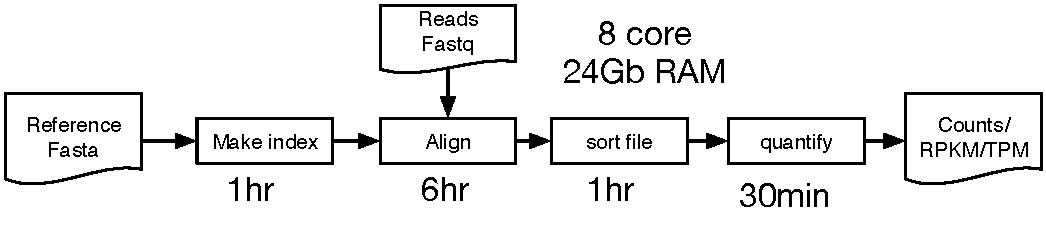
\includegraphics[width=1\textwidth]{expVIP/Figures/alnpipeline.pdf}
\end{subfigure}

\begin{subfigure}{1\textwidth}
\caption{}
\label{fig:exp:mapPipeline}
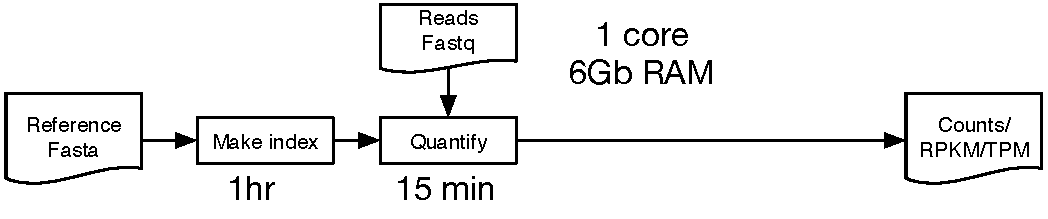
\includegraphics[width=1\textwidth]{expVIP/Figures/mappipeline.pdf}
\end{subfigure}

\caption[Alignment vs mapping pipelines]{Alignment vs mapping pipelines for RNA quantification. (\subref{fig:exp:alnPipeline}) Alignment pipeline. (\subref{fig:exp:mapPipeline}) Mapping pipeline.}
\label{fig:exp:alnVSmap}
\end{figure} 

I decided to integrate \verb|Kallisto|  into expVIP because the algorithm is able to walk through different splicing junctions via a \acrshort{tdbg} (see Section \ref{exp:kallisto}; \citealt{Bray2016}), as opposed to Sailfish, which is based on counting k-mers only \citep{Patro2014}. 
Since homoeologues with a high level of identity may form a bubble in the graph, in a similar way to small indels or SNPs \citep{Leggett2013}, \verb|Kallisto|  should be able to assign the reads to the correct k-compatibility class for their corresponding homoeologue.  
\unsure{Make a diagrame with the graph. Unfortunatly, I don't have in hand my diagrams for cortex an Richard did the diagrams for Legget et al.}

Some features that could improve expVIP in the long term and that already present in other expression browsers would include searching by sequence, by gene ontology and a heatmap of a particular gene displaying two different factors on each axis . 
A feature that expVIP could leverage from other genomic resources is the retrieval of genes flanking a gene of interest, or between genetic markers. 
The upcoming assemblies , from the IWGSC \citep{Clark2016} and TGACv1 \citep{Pozniak2016}  with longer scaffolds in conjunction with the high resolution genetic maps from \citet{Wang2014} and \citet{Chapman2015} can enable such kind of queries (resources described in Section \ref{lit:wheatResourcers}). 

For the TGACv1 assembly, an improved wheat annotation was made available after the initial release of expVIP (Figure \ref{fig:exp:timeline}). The \acrshort{iwgsc} will provide an updated annotation for their genome as well. 
In the near future, expVIP will be updated to include those annotations and some development will be needed to allow the comparison between annotations, at least while the community adopts a canonical reference. 

The same mechanisms to compare expression between different references can be used to compare the expression between different organisms. 
However, the current implementation uses the homology table with one column for each genome group in hexaploid wheat (A, B, and D; Figure \ref{fig:exp:currentGeneRelations}). 
To be able to allow the inclusion of different polyploids with different genome names, to compare homologoues and paralogues effectively and to add any arbitrary relationship between genes the homoeologues table needs to be updated. 
Instead of representing triplets, the table should contain binary relationships; each gene pair will have a type to be able to distinguish between relationships. 
Furthermore, each gene set should be linked to a species. 
With that explicit relationship, equivalent genes from the same species, but coming from different gene models can be identified. 
Likewise, genes known to be conserved across relatives (ie Barley vs Wheat genes) can be compared through these modifications to the database (Figure \ref{fig:exp:futureGeneRelations}).  

\begin{figure}
\centering
\begin{subfigure}{0.45\textwidth}
\centering
\caption{}
\label{fig:exp:currentGeneRelations}
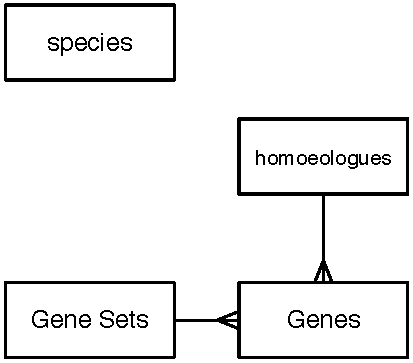
\includegraphics[width=0.85\textwidth]{expVIP/Figures/currentGeneRelations.pdf}
\end{subfigure}
~
\begin{subfigure}{0.45\textwidth}
\centering
\caption{}
\label{fig:exp:futureGeneRelations}
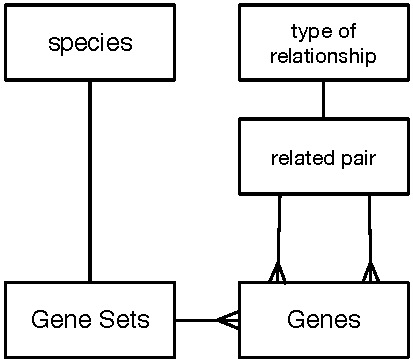
\includegraphics[width=0.85\textwidth]{expVIP/Figures/futureGeneRelations.pdf}
\end{subfigure}
\caption[Changes to improve gene comparasions]{Changes to improve gene comparisons. (\subref{fig:exp:currentGeneRelations}) Current implementation of homoeology. (\subref{fig:exp:currentGeneRelations}) Proposed implementation to extend the types of relationships between genes.  }
\end{figure}

To the best of my knowledge, none of the expression browsers available for wheat, or other polyploid species, allow the direct comparison between homoeologues. However, the effect of different related genes is a topic of active research in polyploids. 
Making the relationship of the expression between related genes easily accessible can provide some initial evidence of having an uniform expression across homoeologues or of a triplet with a dominant gene. 
Likewise, when the update to the table that keeps arbitrary relationships between genes is completed, it will be possible to find if related genes have a conserved expression pattern. 

Since its conception, I wanted expVIP to be open source and available to the community. 
As part of the project, I released the visualisation component as a biojs component  (\texttt{bio-vis-expression-bar}; \url{http://biojs.io/d/bio-vis-expression-bar}; \citealt{Yachdav2015}).
In a collaboration with the Earlham Institute and eLife, another PhD student is working to integrate the visualisation plugin as a live figure. 
If I had kept the code closed, this potential use of the component would have never happened. 

The webserver is also open and hosted on github (\url{https://github.com/homonecloco/expvip-web}), with a tutorial on how to load the data on a personal server (Appendix \ref{exp:tutorial}). 
As the quantification tool used by expVIP has a relatively low memory requirement, I was able to prepare and preconfigure two virtual machines, one without any data loaded and one with all the data used in the original article \url{http://www.wheat-expression.com}. 
This allows the comparison of private projects in the context of previous studies. 
On the Norwich Research Park, at least two groups have shown interest on using expVIP to make their data available to the community on other species.
We had also been contacted by both the team behind the annotation of TGACv1 and the IWGSC to include the upcoming annotations to the public instance of expVIP. 

The public server has received visitors from several research institutes around the globe (Figure \ref{fig:exp:users}). 
Since April, when the google analytics tracker was setup in the website, over 1,500 users have visited the site. 
Most of the users are based in the UK (34\%), and within the nation the majority of the traffic originates from Norwich, Cambridge, Harpenden, London and Dundee. 
Those cities have research institutes that work on wheat, so it is very likely that the users are real. 
Most of the international users are coming from the US, China, Australia, India, Germany and Canada. 
In those countries, most of the visitors also come from cities where wheat institutes are based. 
Furthermore, around half of the sessions stay on the website to access either the the individual genes or the heatmap. 
Around 25\% of the sessions consult their genes using the heatmap, suggesting that they have a list of candidate genes for a trait of interest to select by comparing their expression.

\begin{figure}
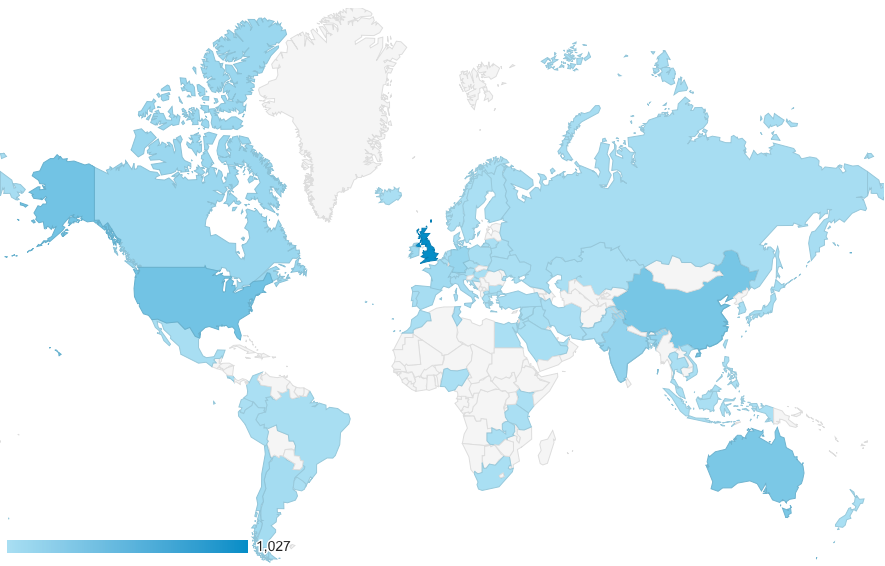
\includegraphics[width=1\textwidth]{expVIP/Figures/WorldSessions.png}
\caption{Heatmap of the number of unique sessions of expVIP in the world.}
\label{fig:exp:users}
\end{figure}

Overall, expVIP has met its aims (Section \ref{exp:aims}). 
I designed a relational database capable of storing several RNA-Seq experiments with their corresponding metadata. 
The expression analysis has been automated, to facilitate the process of running Kallisto, the selected quantification tool. 
The stored data can be visualised to compare the expression across several conditions, and the visualisation tool allows the arbitrary grouping and selection of studies. 
Finally, the open source code and the virtual machines facilitate the adoption of expVIP on other communities, not necessarily working on wheat. 
